\documentclass[11pt,a4paper]{article}
\usepackage[utf8]{inputenc}
\usepackage{amsmath}
\usepackage{amsfonts}
\usepackage{amssymb}
\usepackage{xcolor}
\usepackage{array,booktabs}
\usepackage[none]{hyphenat}
\usepackage{geometry}
\usepackage{graphicx}
\geometry{margin=2.5cm}
\usepackage{float}
\usepackage{multirow}
\usepackage{amsthm}
\usepackage{hyperref}
\theoremstyle{plain}
\usepackage{graphicx}
\usepackage{caption}
\usepackage{subcaption}
\newtheorem{thm}{Theorem}[section] % reset theorem numbering for each chapter

\theoremstyle{definition}
\newtheorem{defn}[thm]{Definition} % definition numbers are dependent on theorem numbers
\newtheorem{exmp}[thm]{Example} % same for example numbers
%\usepackage{cmbright}
\usepackage{fancyhdr}
\pagestyle{fancy}
\fancyhf{}
\rhead{Biharmonic Test}
\lhead{\leftmark}
\rfoot{\thepage}
\author{}
\title{}
\begin{document}
In this tests we consider:
\begin{itemize}
\item $\psi(x)=x^4$
\item $\psi_\text l=0$
\item $\psi_\text r=1$
\item $\psi_\text{ll}=0$
\item $\psi_\text{rr}=4$
\item $g(x)=-24$
\end{itemize}
\begin{table}[H]
\setlength{\tabcolsep}{5pt}
\centering
\caption{Numerical results of PRO1 scheme.}
\resizebox{\linewidth}{!}{%
  \begin{tabular}{@{}l c c c c c c c c c c c c@{}}
\toprule
&  & \multicolumn{2}{c}{$\omega=1|1,1$} &  & \multicolumn{2}{c}{$\omega=1|3,1$} &  & \multicolumn{2}{c}{$\omega=1|3,3$} &  & \multicolumn{2}{c}{$\omega=1|3,10$} \\
\cline{3-4} \cline{6-7} \cline{9-10} \cline{12-13}
 & $I$ & E$_{\infty,0}$ & O$_{\infty,0}$ &  & E$_{\infty,0}$ & O$_{\infty,0}$ &  & E$_{\infty,0}$ & O$_{\infty,0}$ &  & E$_{\infty,0}$ & O$_{\infty,0}$ \\
\midrule
\multirow{6}{*}{$\mathbb{P}_{3}$(4)}
 & 20 & 3.33E$-$03 & ---  &  & 2.51E$-$03 & --- &  & 2.51E$-$03 & --- &  & 2.51E$-$03 & ---\\
 & 40 & 4.31E$-$04 & 2.95  &  & 3.21E$-$04 & 2.97 &  & 3.21E$-$04 & 2.97 &  & 3.21E$-$04 & 2.97\\
 & 80 & 5.46E$-$05 & 2.98  &  & 4.04E$-$05 & 2.99 &  & 4.04E$-$05 & 2.99 &  & 4.04E$-$05 & 2.99\\
 & 160 & 6.86E$-$06 & 2.99  &  & 5.07E$-$06 & 2.99 &  & 5.07E$-$06 & 2.99 &  & 5.07E$-$06 & 2.99\\
 & 320 & 8.59E$-$07 & 3.00  &  & 6.35E$-$07 & 3.00 &  & 6.35E$-$07 & 3.00 &  & 6.35E$-$07 & 3.00\\
 & 640 & 1.08E$-$07 & 3.00  &  & 7.85E$-$08 & 3.02 &  & 7.78E$-$08 & 3.03 &  & 7.92E$-$08 & 3.00\\
\midrule
\multirow{6}{*}{$\mathbb{P}_{5}$(6)}
 & 20 & 9.04E$-$15 & ---  &  & 8.46E$-$14 & --- &  & 1.06E$-$14 & --- &  & 7.08E$-$14 & ---\\
 & 40 & 1.90E$-$13 & $\uparrow$  &  & 6.23E$-$14 & 0.44 &  & 9.63E$-$13 & $\uparrow$ &  & 1.23E$-$13 & $\uparrow$\\
 & 80 & 9.53E$-$13 & $\uparrow$  &  & 6.88E$-$12 & $\uparrow$ &  & 5.70E$-$13 & 0.76 &  & 3.56E$-$12 & $\uparrow$\\
 & 160 & 9.30E$-$12 & $\uparrow$  &  & 1.39E$-$11 & $\uparrow$ &  & 3.07E$-$11 & $\uparrow$ &  & 3.49E$-$11 & $\uparrow$\\
 & 320 & 4.35E$-$11 & $\uparrow$  &  & 6.27E$-$11 & $\uparrow$ &  & 1.61E$-$10 & $\uparrow$ &  & 4.95E$-$11 & $\uparrow$\\
 & 640 & 1.12E$-$09 & $\uparrow$  &  & 1.88E$-$09 & $\uparrow$ &  & 5.79E$-$09 & $\uparrow$ &  & 7.56E$-$10 & $\uparrow$\\
\bottomrule
\end{tabular}}
\label{PRO:bending:01_01_glob3_pro1}
\end{table}

\begin{table}[H]
\setlength{\tabcolsep}{5pt}
\centering
\caption{Numerical results of PRO1 scheme (consistency).}
\resizebox{\linewidth}{!}{%
  \begin{tabular}{@{}l c c c c c c c c c c c c@{}}
\toprule
&  & \multicolumn{2}{c}{$\omega=1|1,1$} &  & \multicolumn{2}{c}{$\omega=1|3,1$} &  & \multicolumn{2}{c}{$\omega=1|3,3$} &  & \multicolumn{2}{c}{$\omega=1|3,10$} \\
\cline{3-4} \cline{6-7} \cline{9-10} \cline{12-13}
 & $I$ & E$_{\infty,0}$ & O$_{\infty,0}$ &  & E$_{\infty,0}$ & O$_{\infty,0}$ &  & E$_{\infty,0}$ & O$_{\infty,0}$ &  & E$_{\infty,0}$ & O$_{\infty,0}$ \\
\midrule
\multirow{6}{*}{$\mathbb{P}_{3}$(4)}
 & 20 & 1.65E$+$01 & ---  &  & 1.67E$+$01 & --- &  & 1.67E$+$01 & --- &  & 1.67E$+$01 & ---\\
 & 40 & 1.65E$+$01 & 0.00  &  & 1.67E$+$01 & 0.00 &  & 1.67E$+$01 & 0.00 &  & 1.67E$+$01 & 0.00\\
 & 80 & 1.65E$+$01 & 0.00  &  & 1.67E$+$01 & 0.00 &  & 1.67E$+$01 & 0.00 &  & 1.67E$+$01 & 0.00\\
 & 160 & 1.65E$+$01 & 0.00  &  & 1.67E$+$01 & 0.00 &  & 1.67E$+$01 & 0.00 &  & 1.67E$+$01 & 0.00\\
 & 320 & 1.65E$+$01 & 0.00  &  & 1.67E$+$01 & 0.00 &  & 1.67E$+$01 & 0.00 &  & 1.67E$+$01 & 0.00\\
 & 640 & 1.65E$+$01 & 0.00  &  & 1.67E$+$01 & $\uparrow$ &  & 1.67E$+$01 & $\uparrow$ &  & 1.67E$+$01 & $\uparrow$\\
\midrule
\multirow{6}{*}{$\mathbb{P}_{5}$(6)}
 & 20 & 1.50E$-$09 & ---  &  & 7.49E$-$10 & --- &  & 4.75E$-$10 & --- &  & 1.08E$-$09 & ---\\
 & 40 & 5.87E$-$09 & $\uparrow$  &  & 1.90E$-$08 & $\uparrow$ &  & 2.36E$-$08 & $\uparrow$ &  & 3.87E$-$08 & $\uparrow$\\
 & 80 & 9.32E$-$08 & $\uparrow$  &  & 2.28E$-$07 & $\uparrow$ &  & 2.14E$-$07 & $\uparrow$ &  & 3.22E$-$07 & $\uparrow$\\
 & 160 & 2.08E$-$06 & $\uparrow$  &  & 1.61E$-$06 & $\uparrow$ &  & 2.75E$-$06 & $\uparrow$ &  & 2.24E$-$06 & $\uparrow$\\
 & 320 & 1.27E$-$05 & $\uparrow$  &  & 7.75E$-$06 & $\uparrow$ &  & 1.75E$-$05 & $\uparrow$ &  & 1.13E$-$04 & $\uparrow$\\
 & 640 & 1.86E$-$04 & $\uparrow$  &  & 3.24E$-$04 & $\uparrow$ &  & 1.71E$-$04 & $\uparrow$ &  & 3.12E$-$04 & $\uparrow$\\
\bottomrule
\end{tabular}}
\label{PRO:bending:01_01_glob3_pro1_cons}
\end{table}


\begin{figure}[H]
\begin{subfigure}[b]{0.48\textwidth}
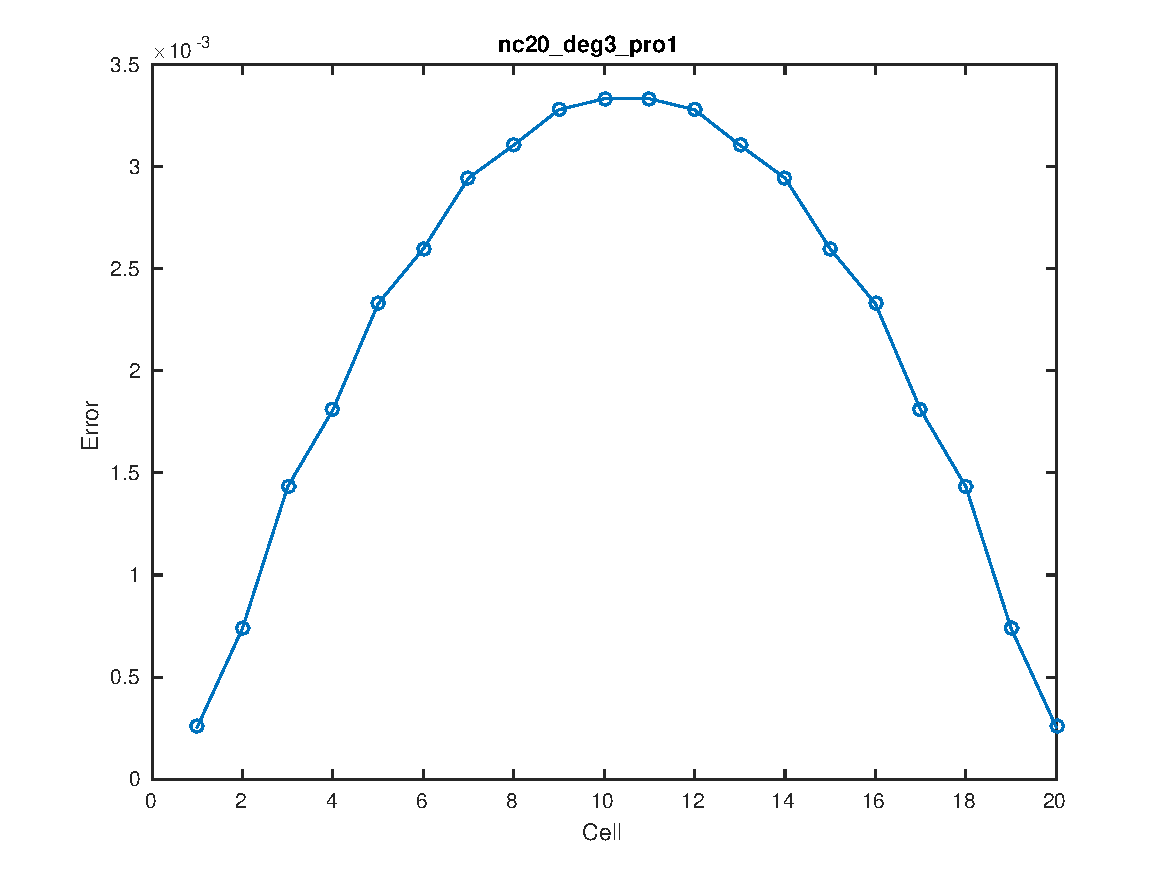
\includegraphics[width=\linewidth]{../../tests_01_01/test_01_01_test9_pro1/output/plots/nc20_deg3_wei111_pro1.pdf}
\end{subfigure}\hspace*{\fill}
\begin{subfigure}[b]{0.48\textwidth}
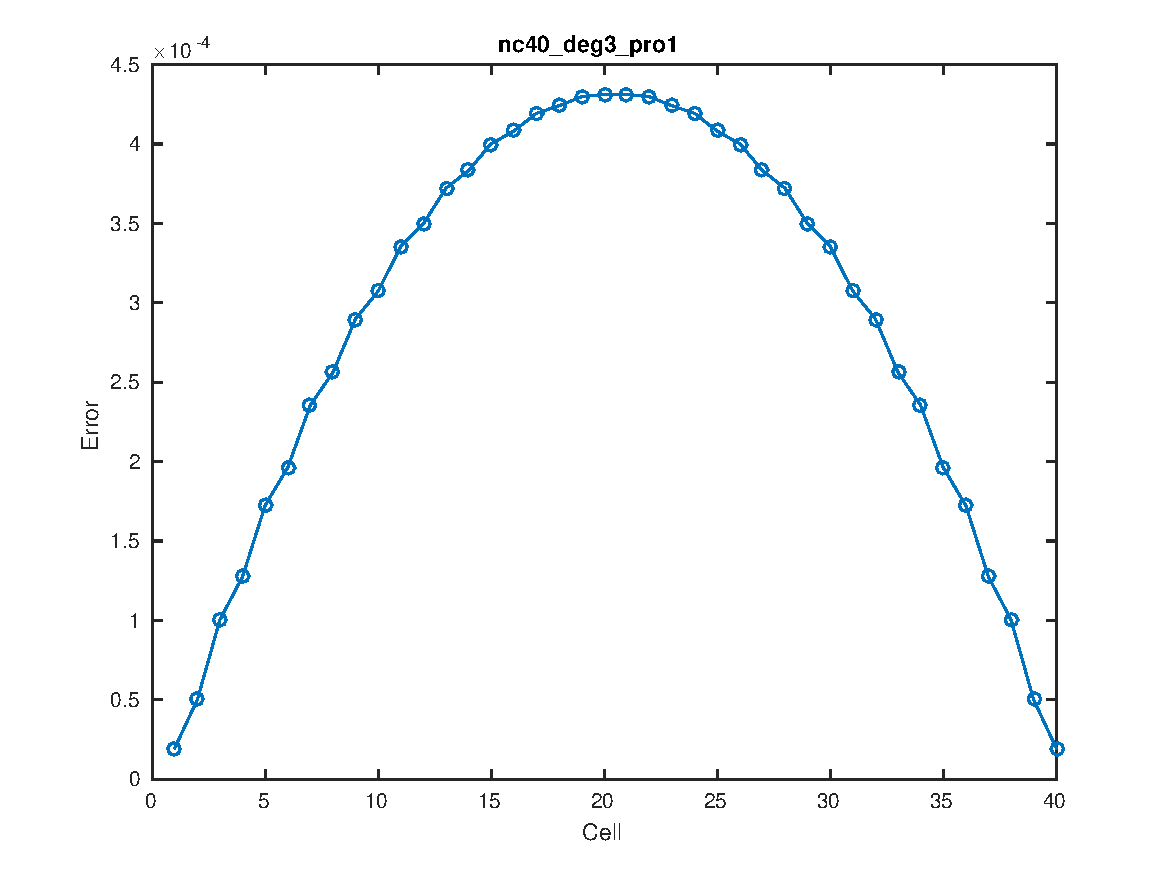
\includegraphics[width=\linewidth]{../../tests_01_01/test_01_01_test9_pro1/output/plots/nc40_deg3_wei111_pro1.pdf}
\end{subfigure}

\medskip
\begin{subfigure}[b]{0.48\textwidth}
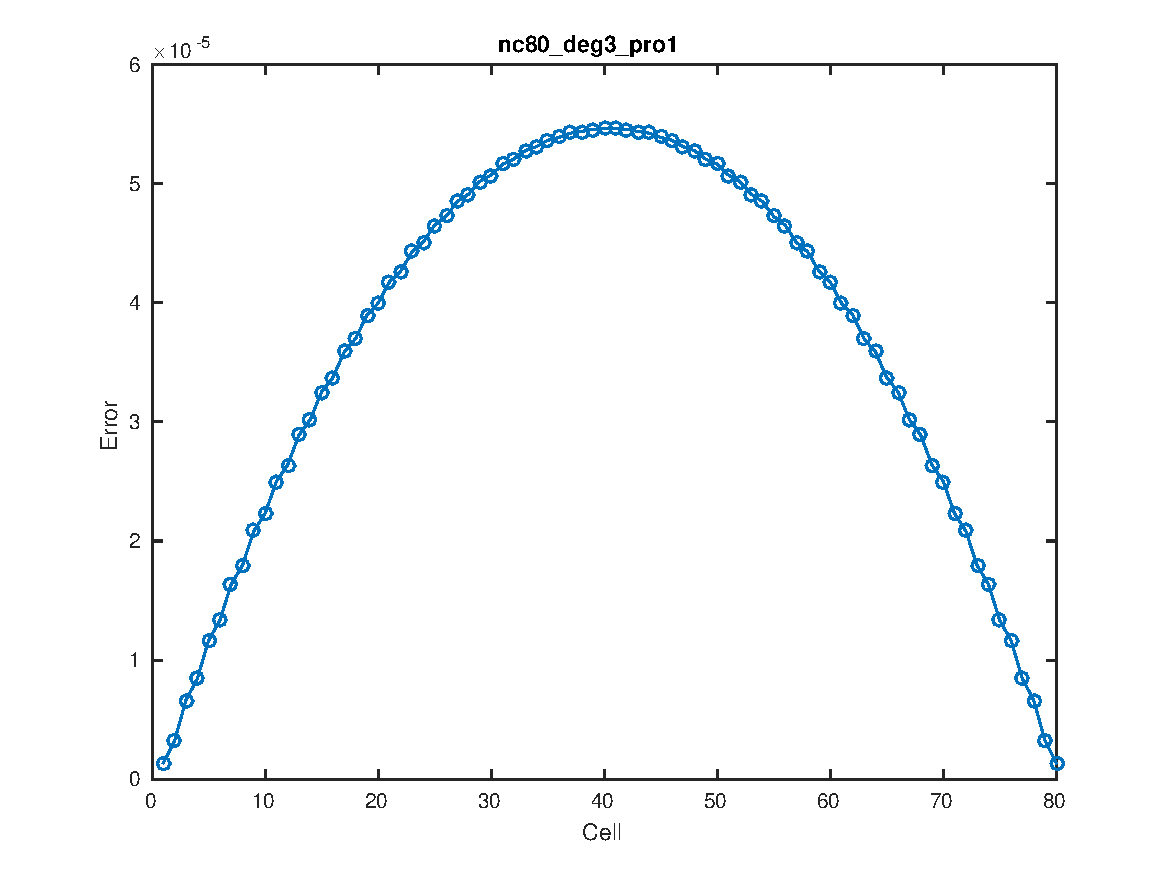
\includegraphics[width=\linewidth]{../../tests_01_01/test_01_01_test9_pro1/output/plots/nc80_deg3_wei111_pro1.pdf}
\end{subfigure}\hspace*{\fill}
\begin{subfigure}[b]{0.48\textwidth}
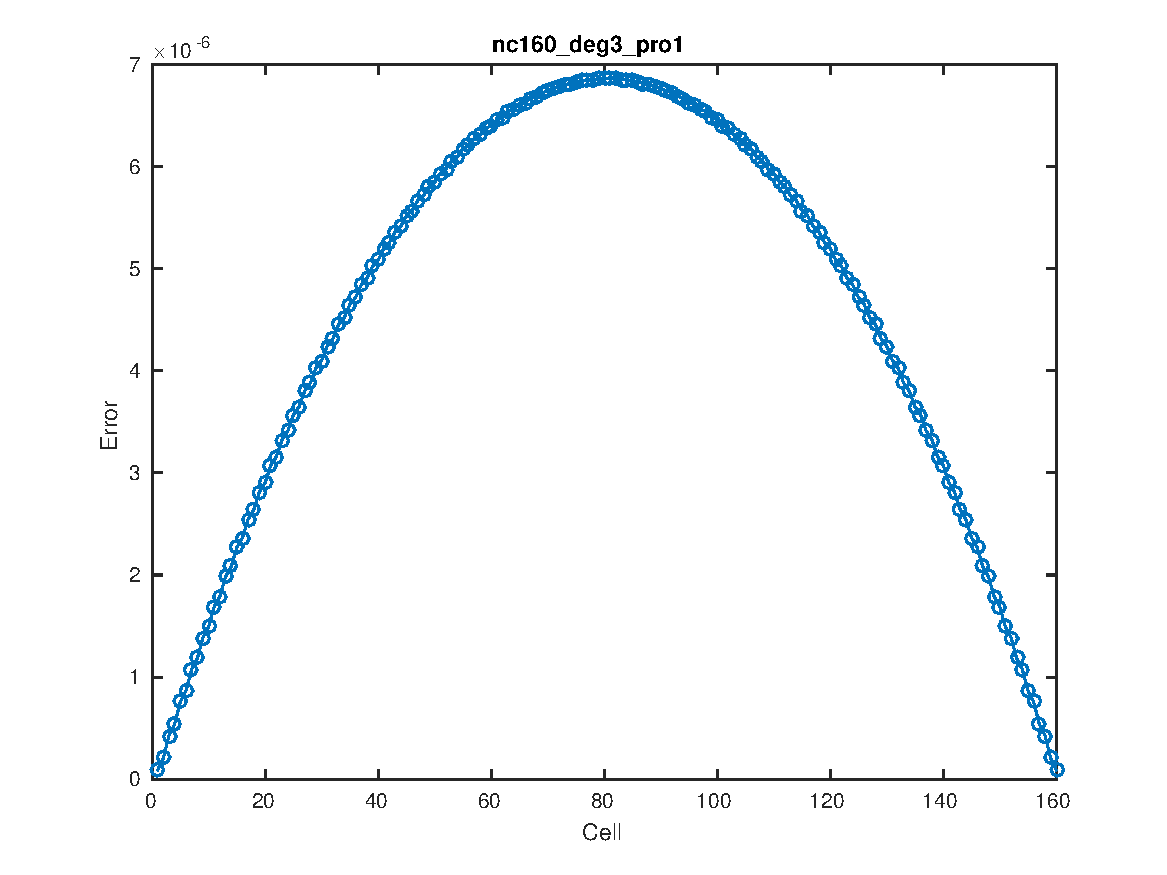
\includegraphics[width=\linewidth]{../../tests_01_01/test_01_01_test9_pro1/output/plots/nc160_deg3_wei111_pro1.pdf}
\end{subfigure}

\medskip
\begin{subfigure}[b]{0.48\textwidth}
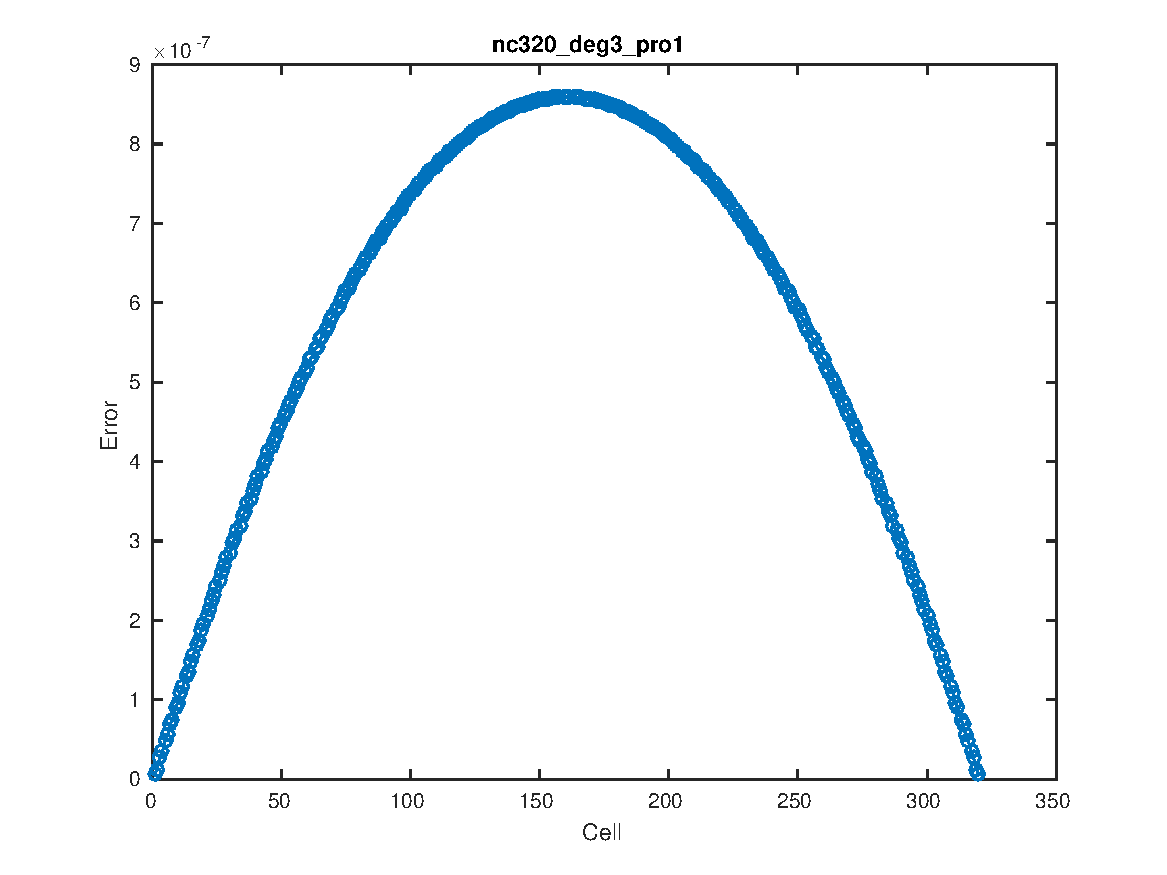
\includegraphics[width=\linewidth]{../../tests_01_01/test_01_01_test9_pro1/output/plots/nc320_deg3_wei111_pro1.pdf}
\end{subfigure}\hspace*{\fill}
\begin{subfigure}[b]{0.48\textwidth}
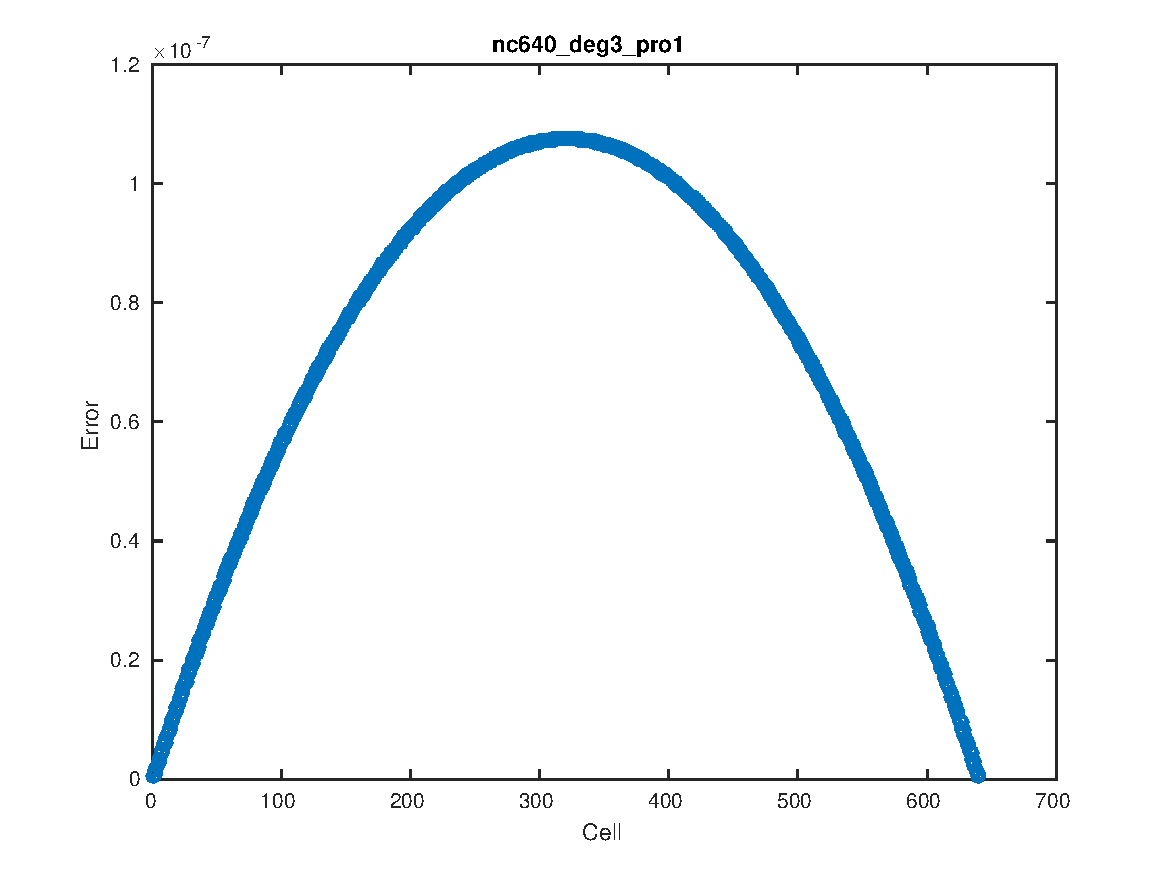
\includegraphics[width=\linewidth]{../../tests_01_01/test_01_01_test9_pro1/output/plots/nc640_deg3_wei111_pro1.pdf}
\end{subfigure}

\caption{$\omega=1|1,1$, d=3}
\end{figure}
%%%% 2
\begin{figure}[H]
\begin{subfigure}[b]{0.48\textwidth}
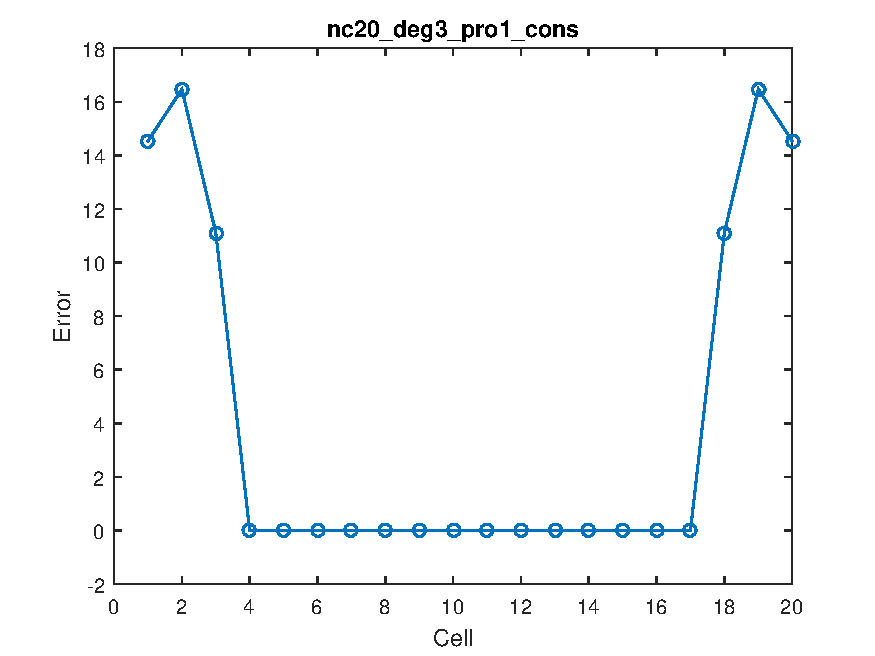
\includegraphics[width=\linewidth]{../../tests_01_01/test_01_01_test9_pro1_cons/output/plots/nc20_deg3_wei111_pro1_cons.pdf}
\end{subfigure}\hspace*{\fill}
\begin{subfigure}[b]{0.48\textwidth}
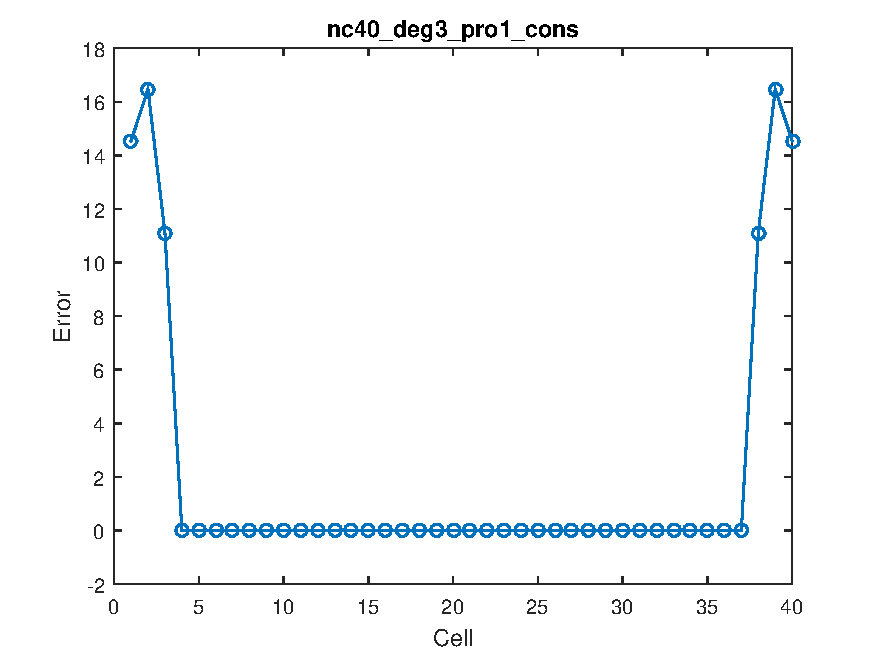
\includegraphics[width=\linewidth]{../../tests_01_01/test_01_01_test9_pro1_cons/output/plots/nc40_deg3_wei111_pro1_cons.pdf}
\end{subfigure}

\medskip
\begin{subfigure}[b]{0.48\textwidth}
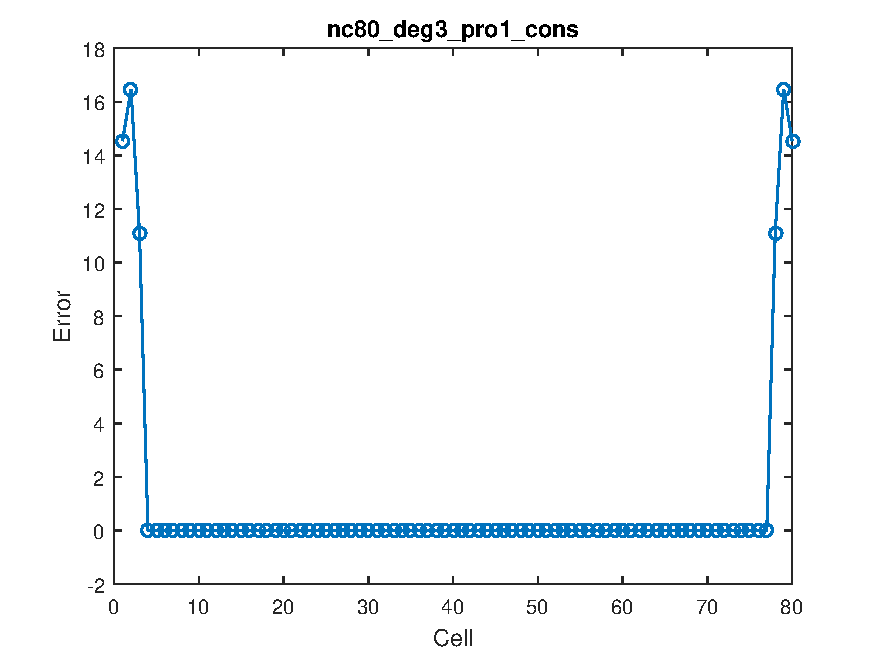
\includegraphics[width=\linewidth]{../../tests_01_01/test_01_01_test9_pro1_cons/output/plots/nc80_deg3_wei111_pro1_cons.pdf}
\end{subfigure}\hspace*{\fill}
\begin{subfigure}[b]{0.48\textwidth}
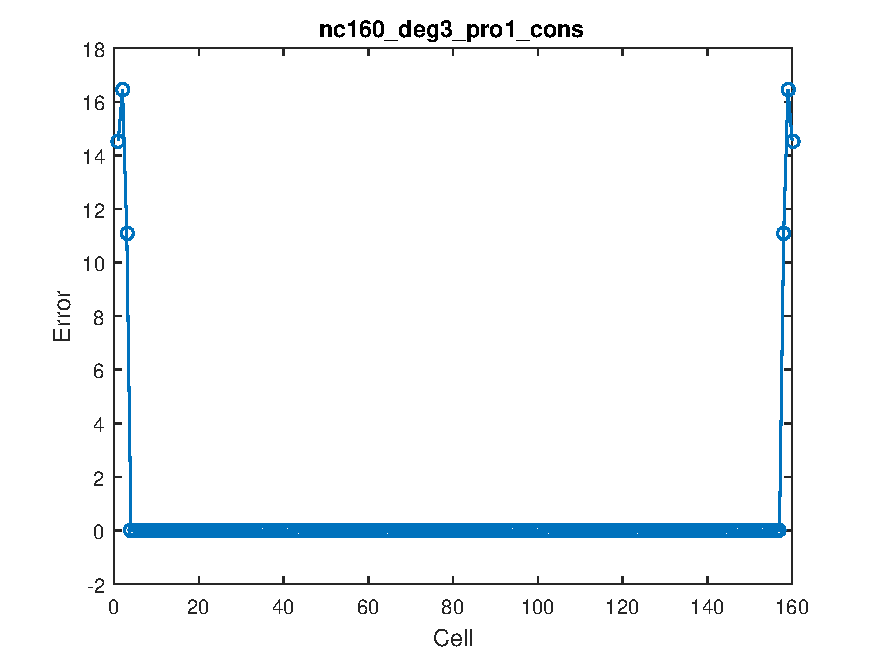
\includegraphics[width=\linewidth]{../../tests_01_01/test_01_01_test9_pro1_cons/output/plots/nc160_deg3_wei111_pro1_cons.pdf}
\end{subfigure}

\medskip
\begin{subfigure}[b]{0.48\textwidth}
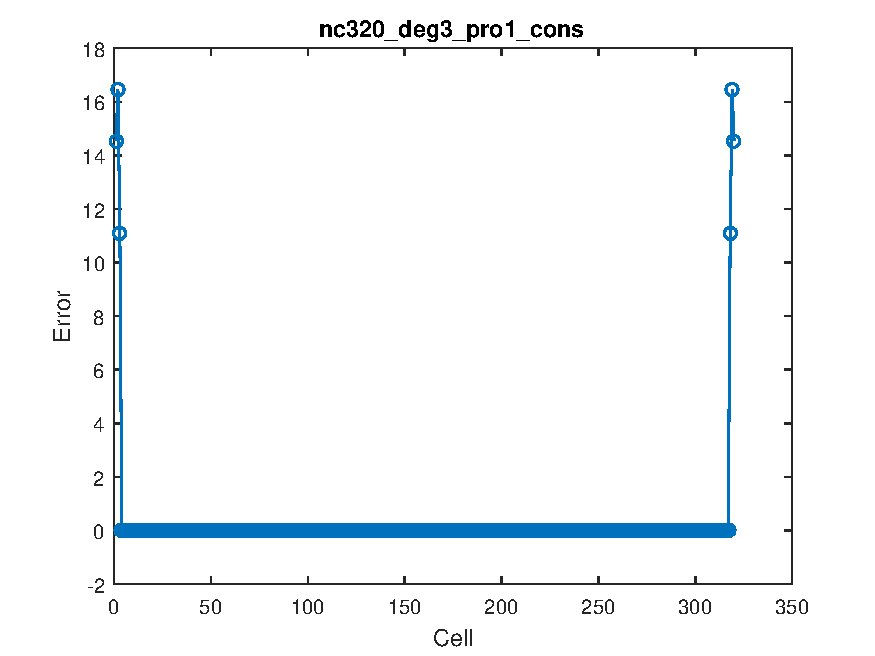
\includegraphics[width=\linewidth]{../../tests_01_01/test_01_01_test9_pro1_cons/output/plots/nc320_deg3_wei111_pro1_cons.pdf}
\end{subfigure}\hspace*{\fill}
\begin{subfigure}[b]{0.48\textwidth}
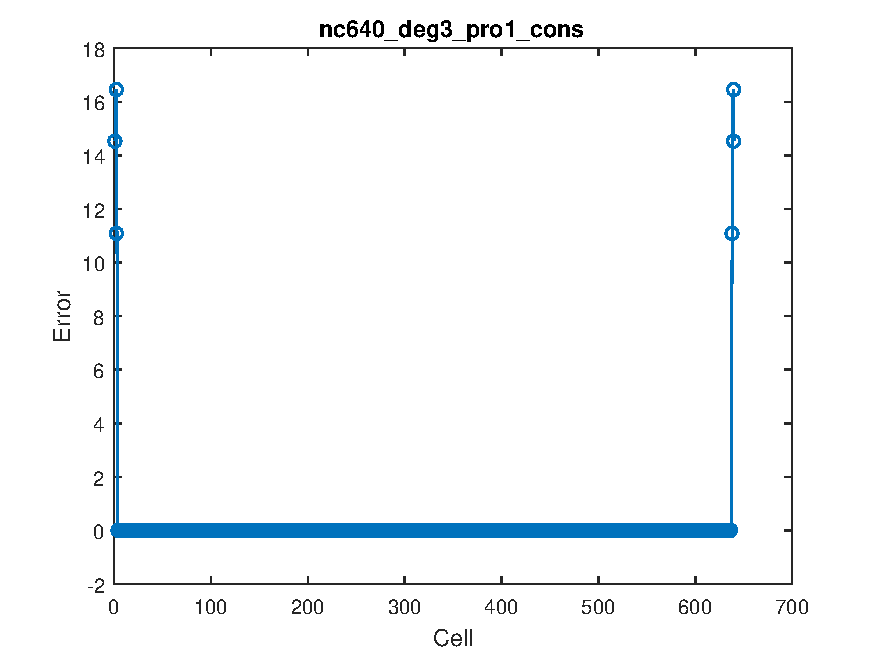
\includegraphics[width=\linewidth]{../../tests_01_01/test_01_01_test9_pro1_cons/output/plots/nc640_deg3_wei111_pro1_cons.pdf}
\end{subfigure}

\caption{$\omega=1|1,1$, d=3 (consistency)}
\end{figure}
%%%% 3
\begin{figure}[H]
\begin{subfigure}[b]{0.48\textwidth}
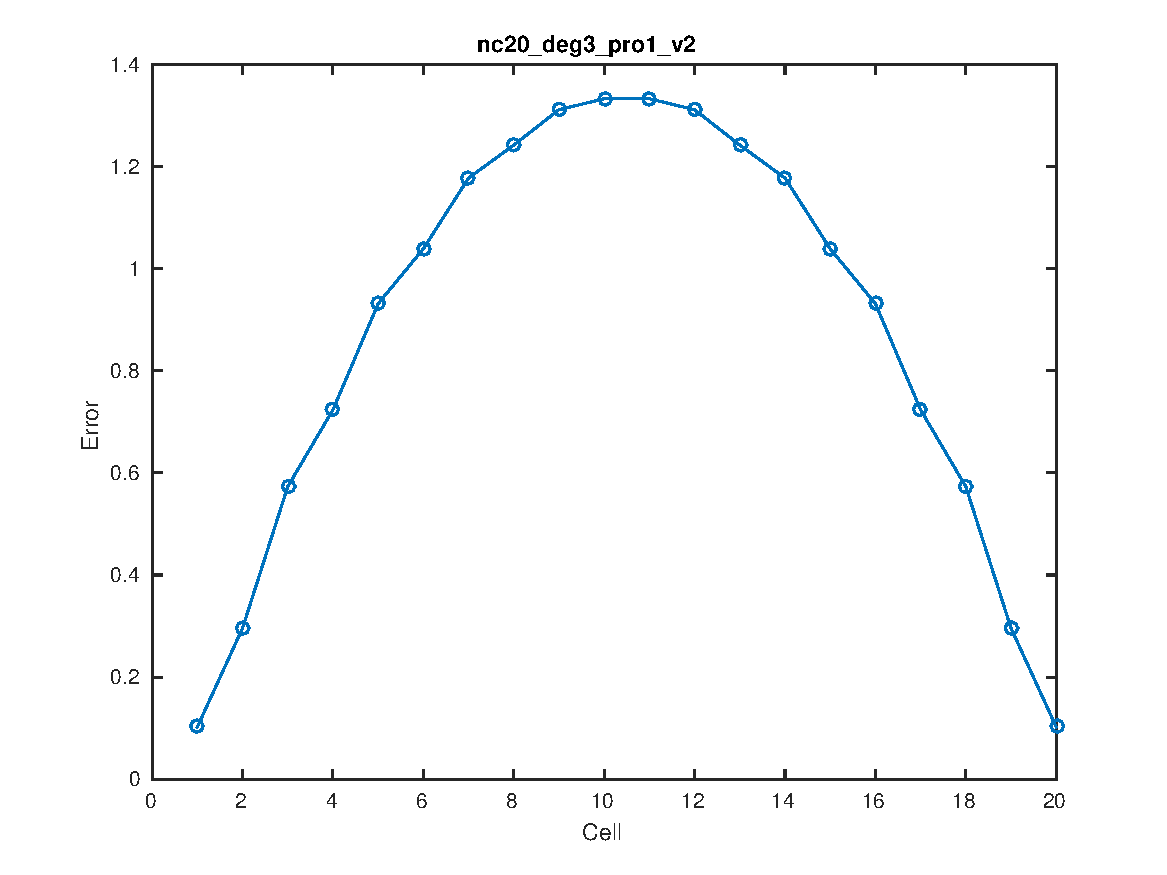
\includegraphics[width=\linewidth]{../../tests_01_01/test_01_01_test9_pro1/output/plots/nc20_deg3_wei111_pro1_v2.pdf}
\end{subfigure}\hspace*{\fill}
\begin{subfigure}[b]{0.48\textwidth}
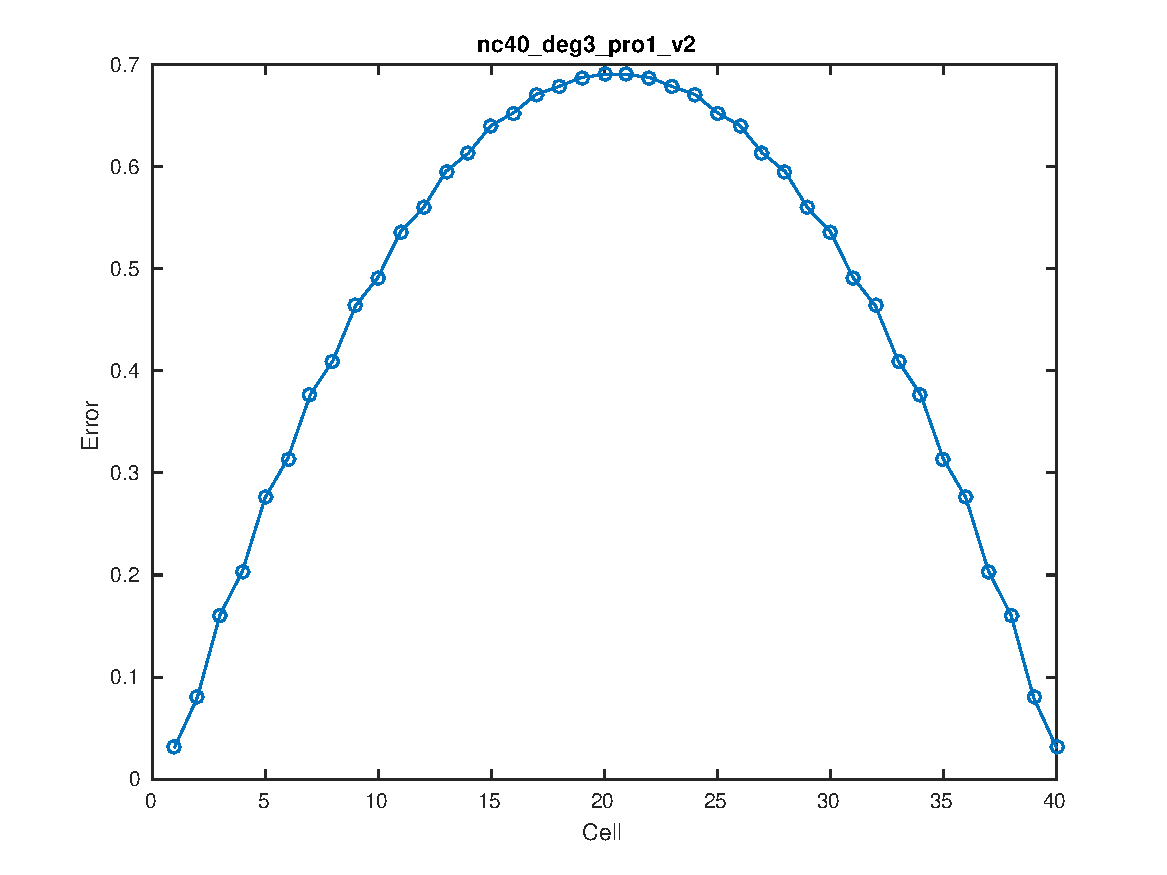
\includegraphics[width=\linewidth]{../../tests_01_01/test_01_01_test9_pro1/output/plots/nc40_deg3_wei111_pro1_v2.pdf}
\end{subfigure}

\medskip
\begin{subfigure}[b]{0.48\textwidth}
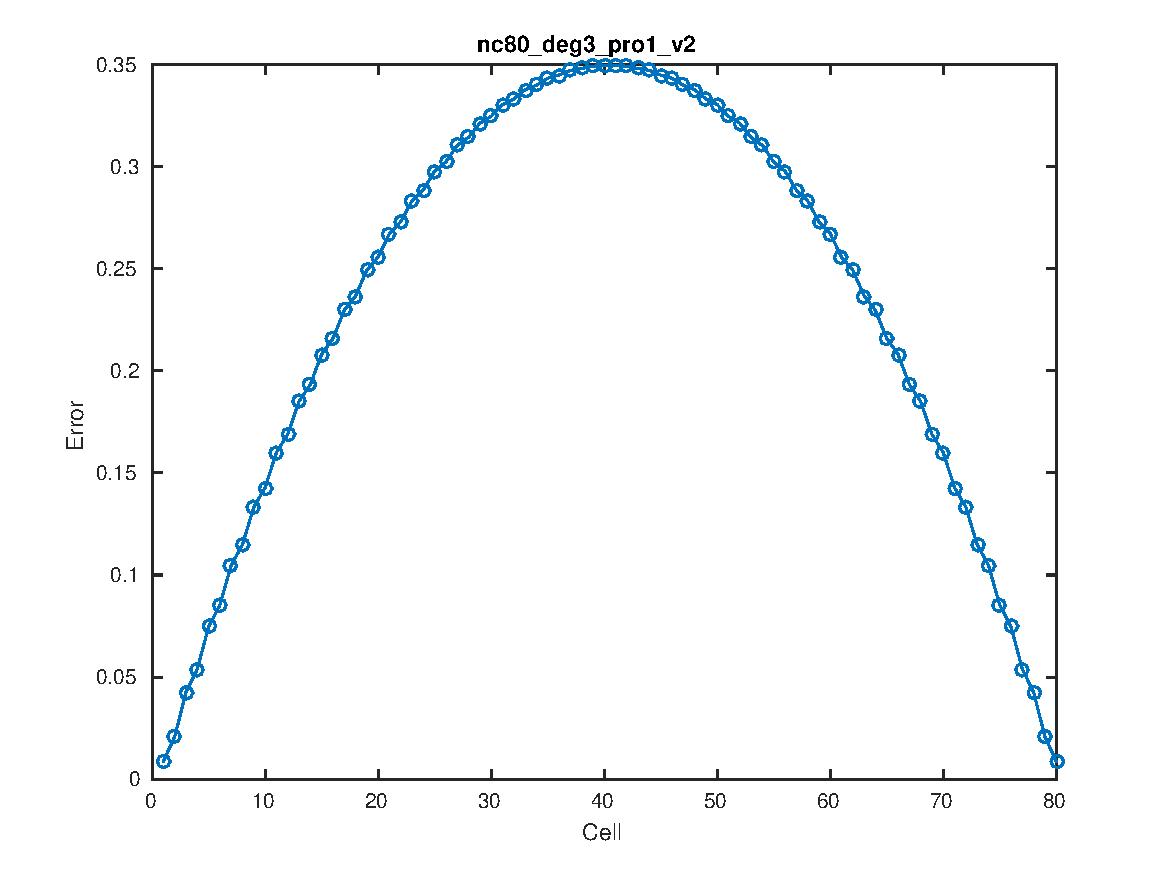
\includegraphics[width=\linewidth]{../../tests_01_01/test_01_01_test9_pro1/output/plots/nc80_deg3_wei111_pro1_v2.pdf}
\end{subfigure}\hspace*{\fill}
\begin{subfigure}[b]{0.48\textwidth}
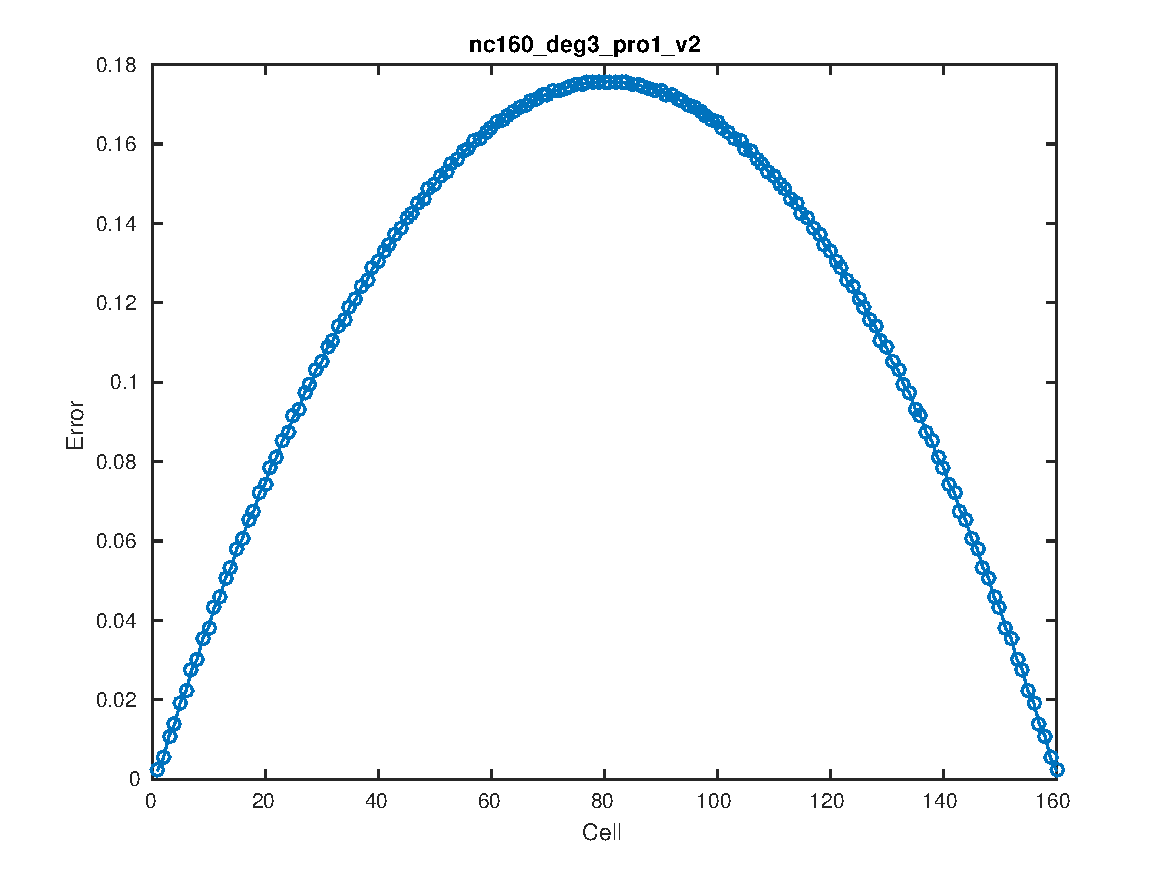
\includegraphics[width=\linewidth]{../../tests_01_01/test_01_01_test9_pro1/output/plots/nc160_deg3_wei111_pro1_v2.pdf}
\end{subfigure}

\medskip
\begin{subfigure}[b]{0.48\textwidth}
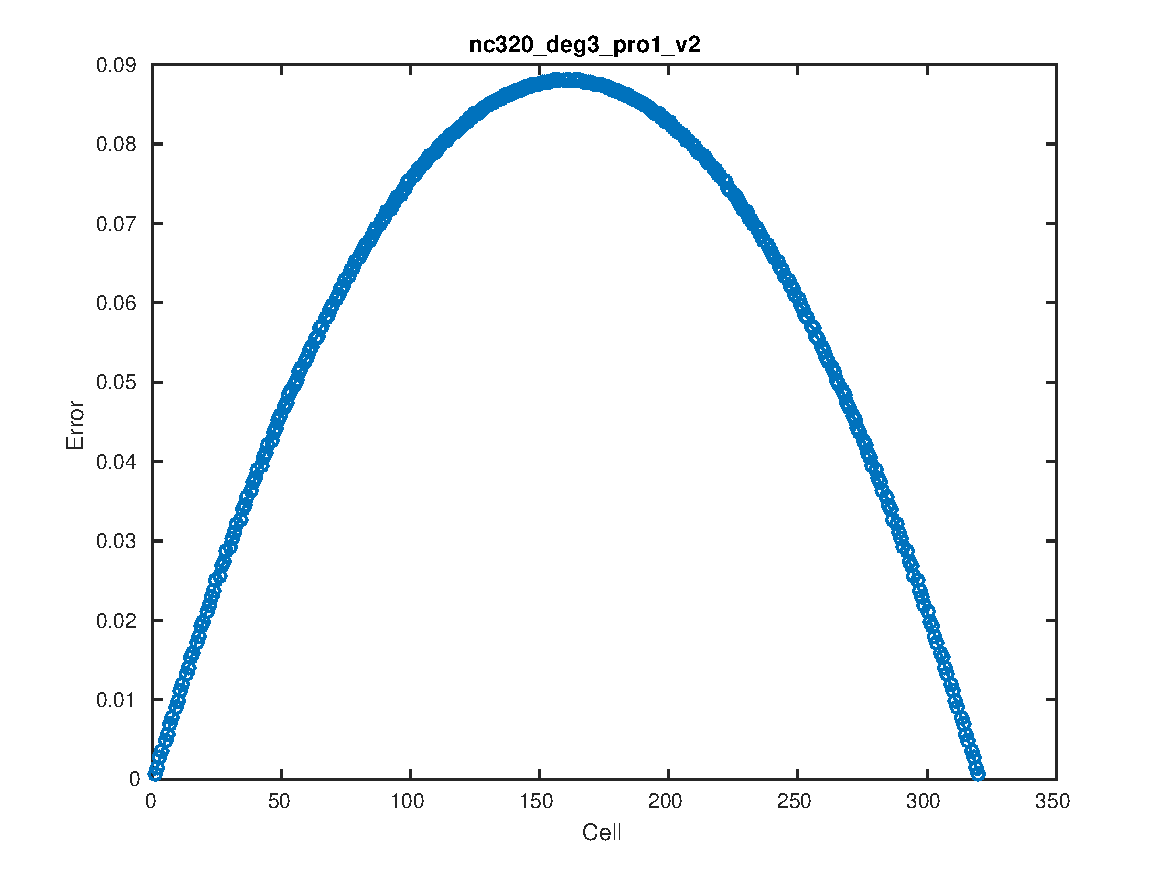
\includegraphics[width=\linewidth]{../../tests_01_01/test_01_01_test9_pro1/output/plots/nc320_deg3_wei111_pro1_v2.pdf}
\end{subfigure}\hspace*{\fill}
\begin{subfigure}[b]{0.48\textwidth}
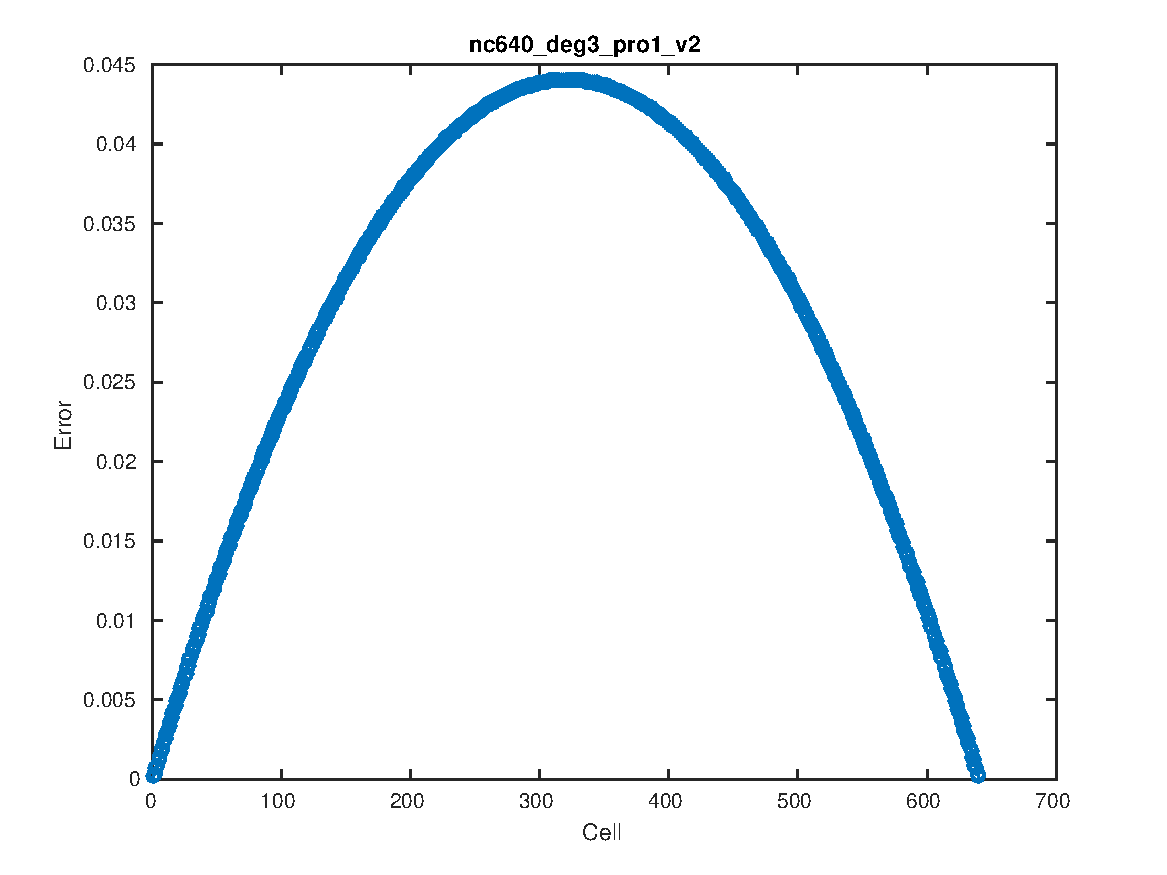
\includegraphics[width=\linewidth]{../../tests_01_01/test_01_01_test9_pro1/output/plots/nc640_deg3_wei111_pro1_v2.pdf}
\end{subfigure}

\caption{$\omega=1|1,1$, d=3  $\left(\frac{x-\overline{x}}{h^2}\right)$}
\end{figure}

\pagebreak
%%%%%%%%%%%%%%%%%%%%%%%%%%%%%%%%%%%%%%%%%%%%%%%%%%%%%%%%%%%%%%%%%%%%%%%%%%%%%%%%%%%%%%%%%%
In this tests we consider:
\begin{itemize}
\item $\psi(x)=\exp(x)$
\item $\psi_\text l=1$
\item $\psi_\text r=e$
\item $\psi_\text{ll}=1$
\item $\psi_\text{rr}=e$
\item $g(x)=-\exp(x)$
\end{itemize}
\begin{table}[H]
\setlength{\tabcolsep}{5pt}
\centering
\caption{Numerical results of PRO1 scheme.}
\resizebox{\linewidth}{!}{%
  \begin{tabular}{@{}l c c c c c c c c c c c c@{}}
\toprule
&  & \multicolumn{2}{c}{$\omega=1|1,1$} &  & \multicolumn{2}{c}{$\omega=1|3,1$} &  & \multicolumn{2}{c}{$\omega=1|3,3$} &  & \multicolumn{2}{c}{$\omega=1|3,10$} \\
\cline{3-4} \cline{6-7} \cline{9-10} \cline{12-13}
 & $I$ & E$_{\infty,0}$ & O$_{\infty,0}$ &  & E$_{\infty,0}$ & O$_{\infty,0}$ &  & E$_{\infty,0}$ & O$_{\infty,0}$ &  & E$_{\infty,0}$ & O$_{\infty,0}$ \\
\midrule
\multirow{6}{*}{$\mathbb{P}_{3}$(4)}
 & 20 & 2.60E$-$04 & ---  &  & 2.07E$-$04 & --- &  & 2.07E$-$04 & --- &  & 2.06E$-$04 & ---\\
 & 40 & 3.35E$-$05 & 2.95  &  & 2.65E$-$05 & 2.96 &  & 2.65E$-$05 & 2.96 &  & 2.65E$-$05 & 2.96\\
 & 80 & 4.14E$-$06 & 3.02  &  & 3.27E$-$06 & 3.02 &  & 3.27E$-$06 & 3.02 &  & 3.27E$-$06 & 3.02\\
 & 160 & 4.90E$-$07 & 3.08  &  & 3.82E$-$07 & 3.10 &  & 3.82E$-$07 & 3.10 &  & 3.82E$-$07 & 3.10\\
 & 320 & 5.37E$-$08 & 3.19  &  & 4.08E$-$08 & 3.23 &  & 4.07E$-$08 & 3.23 &  & 4.07E$-$08 & 3.23\\
 & 640 & 4.89E$-$09 & 3.46  &  & 3.84E$-$09 & 3.41 &  & 3.68E$-$09 & 3.47 &  & 3.36E$-$09 & 3.60\\
\midrule
\multirow{6}{*}{$\mathbb{P}_{5}$(6)}
 & 20 & 1.78E$-$07 & ---  &  & 1.48E$-$07 & --- &  & 1.48E$-$07 & --- &  & 1.48E$-$07 & ---\\
 & 40 & 5.36E$-$09 & 5.05  &  & 4.46E$-$09 & 5.06 &  & 4.46E$-$09 & 5.06 &  & 4.46E$-$09 & 5.06\\
 & 80 & 1.56E$-$10 & 5.11  &  & 1.41E$-$10 & 4.98 &  & 1.40E$-$10 & 4.99 &  & 1.38E$-$10 & 5.01\\
 & 160 & 3.10E$-$12 & 5.65  &  & 5.96E$-$12 & 4.57 &  & 2.20E$-$12 & 5.99 &  & 1.21E$-$11 & 3.51\\
 & 320 & 3.84E$-$11 & $\uparrow$  &  & 5.59E$-$11 & $\uparrow$ &  & 1.97E$-$10 & $\uparrow$ &  & 7.13E$-$11 & $\uparrow$\\
 & 640 & 4.06E$-$10 & $\uparrow$  &  & 1.22E$-$09 & $\uparrow$ &  & 1.36E$-$09 & $\uparrow$ &  & 6.03E$-$10 & $\uparrow$\\
\bottomrule
\end{tabular}}
\label{PRO:bending:01_01_glob1_pro1}
\end{table}

\begin{table}[H]
\setlength{\tabcolsep}{5pt}
\centering
\caption{Numerical results of PRO1 scheme (consistency).}
\resizebox{\linewidth}{!}{%
  \begin{tabular}{@{}l c c c c c c c c c c c c@{}}
\toprule
&  & \multicolumn{2}{c}{$\omega=1|1,1$} &  & \multicolumn{2}{c}{$\omega=1|3,1$} &  & \multicolumn{2}{c}{$\omega=1|3,3$} &  & \multicolumn{2}{c}{$\omega=1|3,10$} \\
\cline{3-4} \cline{6-7} \cline{9-10} \cline{12-13}
 & $I$ & E$_{\infty,0}$ & O$_{\infty,0}$ &  & E$_{\infty,0}$ & O$_{\infty,0}$ &  & E$_{\infty,0}$ & O$_{\infty,0}$ &  & E$_{\infty,0}$ & O$_{\infty,0}$ \\
\midrule
\multirow{6}{*}{$\mathbb{P}_{3}$(4)}
 & 20 & 8.75E$-$02 & ---  &  & 9.24E$-$02 & --- &  & 9.24E$-$02 & --- &  & 9.24E$-$02 & ---\\
 & 40 & 4.52E$-$02 & 0.95  &  & 4.58E$-$02 & 1.01 &  & 4.58E$-$02 & 1.01 &  & 4.58E$-$02 & 1.01\\
 & 80 & 2.29E$-$02 & 0.98  &  & 2.33E$-$02 & 0.98 &  & 2.33E$-$02 & 0.98 &  & 2.33E$-$02 & 0.98\\
 & 160 & 1.16E$-$02 & 0.99  &  & 1.17E$-$02 & 0.99 &  & 1.17E$-$02 & 0.99 &  & 1.17E$-$02 & 0.99\\
 & 320 & 5.81E$-$03 & 0.99  &  & 5.89E$-$03 & 0.99 &  & 5.89E$-$03 & 0.99 &  & 5.89E$-$03 & 0.99\\
 & 640 & 2.91E$-$03 & 1.00  &  & 2.95E$-$03 & 1.00 &  & 2.95E$-$03 & 1.00 &  & 2.95E$-$03 & 1.00\\
\midrule
\multirow{6}{*}{$\mathbb{P}_{5}$(6)}
 & 20 & 4.48E$-$04 & ---  &  & 4.68E$-$04 & --- &  & 4.68E$-$04 & --- &  & 4.68E$-$04 & ---\\
 & 40 & 5.84E$-$05 & 2.94  &  & 6.11E$-$05 & 2.94 &  & 6.11E$-$05 & 2.94 &  & 6.11E$-$05 & 2.94\\
 & 80 & 7.46E$-$06 & 2.97  &  & 7.81E$-$06 & 2.97 &  & 7.81E$-$06 & 2.97 &  & 7.81E$-$06 & 2.97\\
 & 160 & 9.30E$-$07 & 3.00  &  & 9.77E$-$07 & 3.00 &  & 9.72E$-$07 & 3.01 &  & 9.89E$-$07 & 2.98\\
 & 320 & 2.49E$-$07 & 1.90  &  & 2.02E$-$07 & 2.27 &  & 2.36E$-$07 & 2.04 &  & 1.48E$-$07 & 2.74\\
 & 640 & 2.09E$-$06 & $\uparrow$  &  & 2.59E$-$06 & $\uparrow$ &  & 2.18E$-$06 & $\uparrow$ &  & 2.03E$-$06 & $\uparrow$\\
\bottomrule
\end{tabular}}
\label{PRO:bending:01_01_glob1_pro1_cons}
\end{table}


\begin{figure}[H]
\begin{subfigure}[b]{0.48\textwidth}
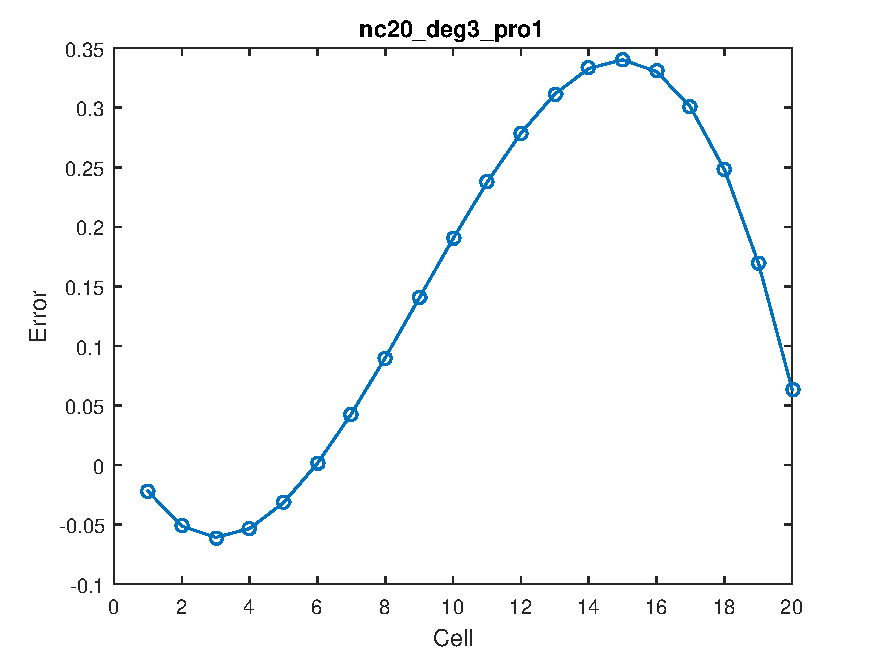
\includegraphics[width=\linewidth]{../../tests_01_01/test_01_01_test1_pro1/output/plots/nc20_deg3_wei111_pro1.pdf}
\end{subfigure}\hspace*{\fill}
\begin{subfigure}[b]{0.48\textwidth}
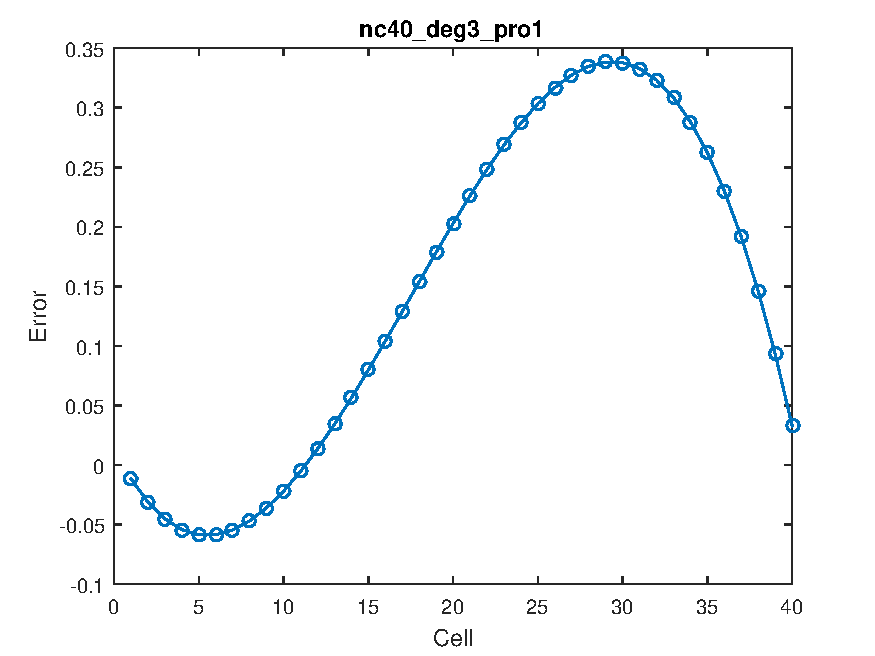
\includegraphics[width=\linewidth]{../../tests_01_01/test_01_01_test1_pro1/output/plots/nc40_deg3_wei111_pro1.pdf}
\end{subfigure}

\medskip
\begin{subfigure}[b]{0.48\textwidth}
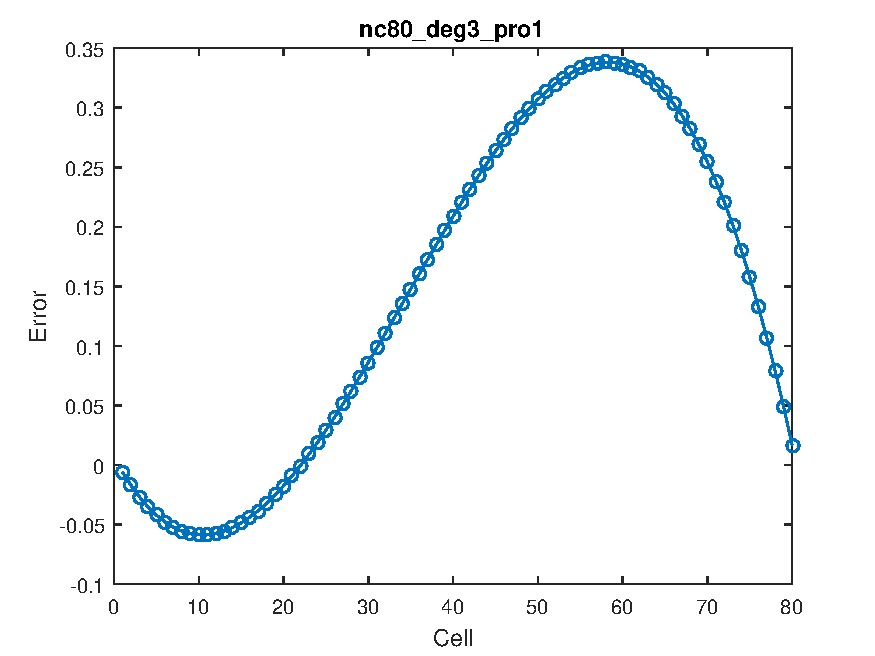
\includegraphics[width=\linewidth]{../../tests_01_01/test_01_01_test1_pro1/output/plots/nc80_deg3_wei111_pro1.pdf}
\end{subfigure}\hspace*{\fill}
\begin{subfigure}[b]{0.48\textwidth}
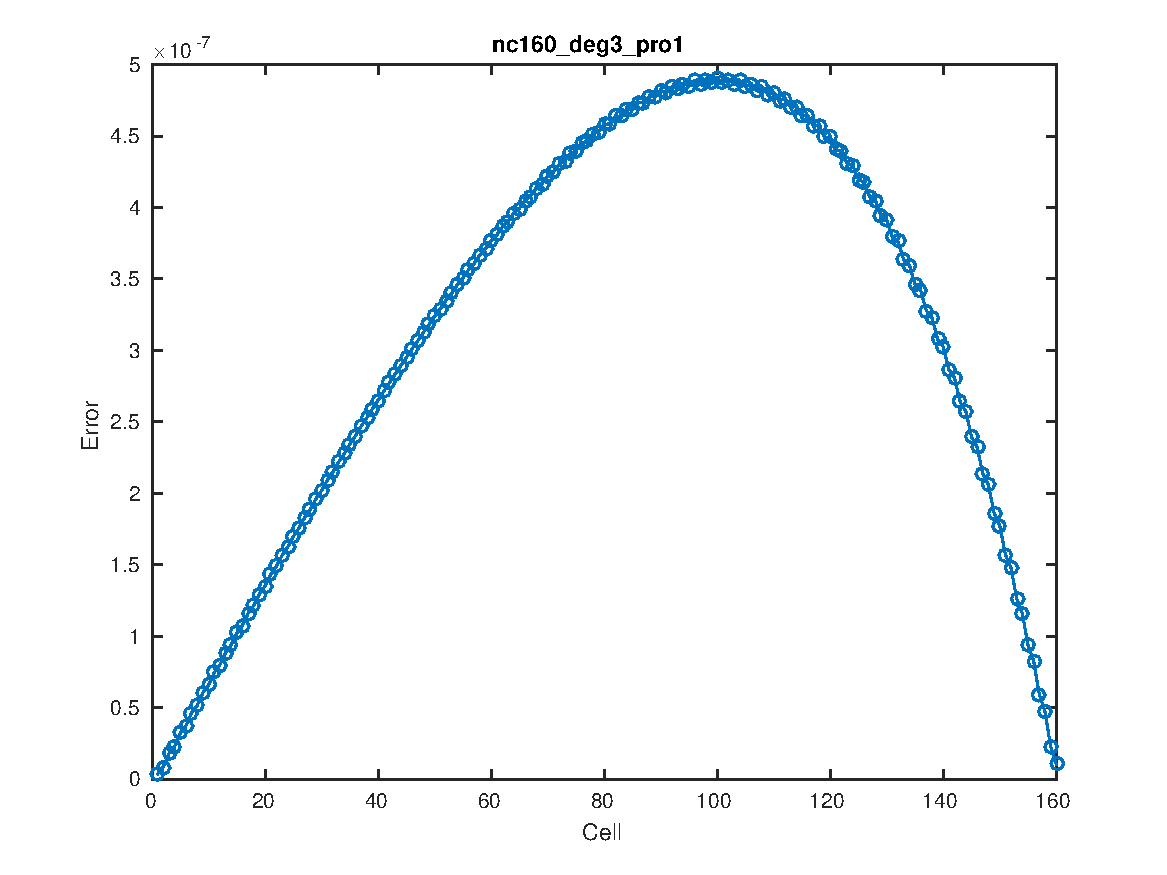
\includegraphics[width=\linewidth]{../../tests_01_01/test_01_01_test1_pro1/output/plots/nc160_deg3_wei111_pro1.pdf}
\end{subfigure}

\medskip
\begin{subfigure}[b]{0.48\textwidth}
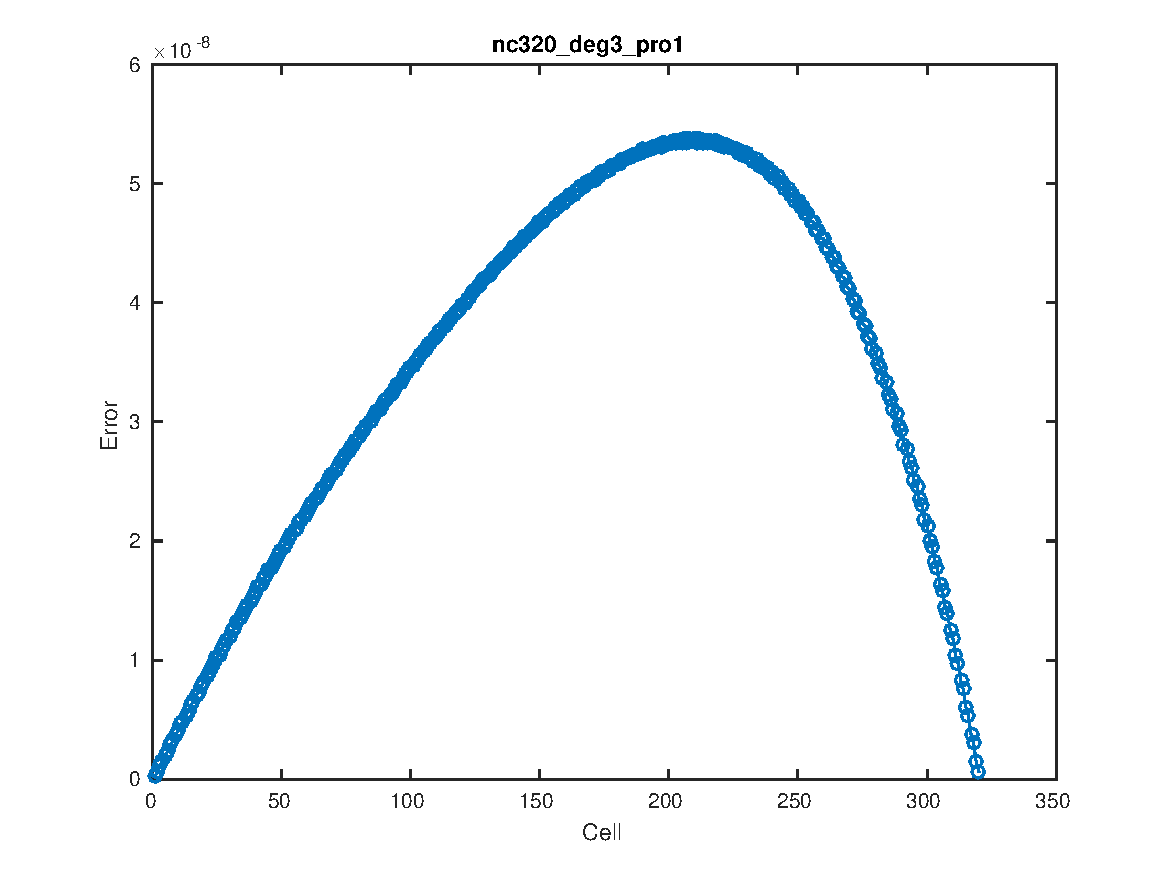
\includegraphics[width=\linewidth]{../../tests_01_01/test_01_01_test1_pro1/output/plots/nc320_deg3_wei111_pro1.pdf}
\end{subfigure}\hspace*{\fill}
\begin{subfigure}[b]{0.48\textwidth}
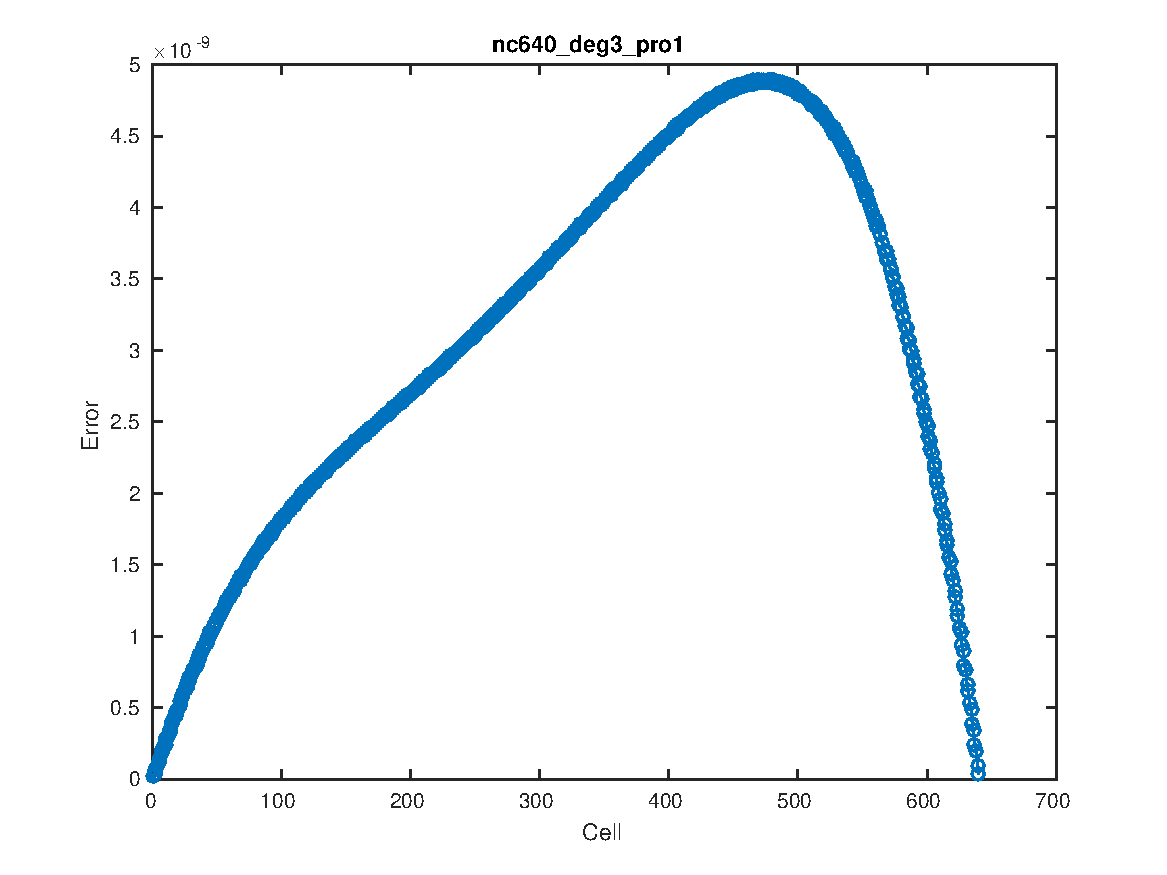
\includegraphics[width=\linewidth]{../../tests_01_01/test_01_01_test1_pro1/output/plots/nc640_deg3_wei111_pro1.pdf}
\end{subfigure}

\caption{$\omega=1|1,1$, d=3}
\end{figure}
%%% 2
\begin{figure}[H]
\begin{subfigure}[b]{0.48\textwidth}
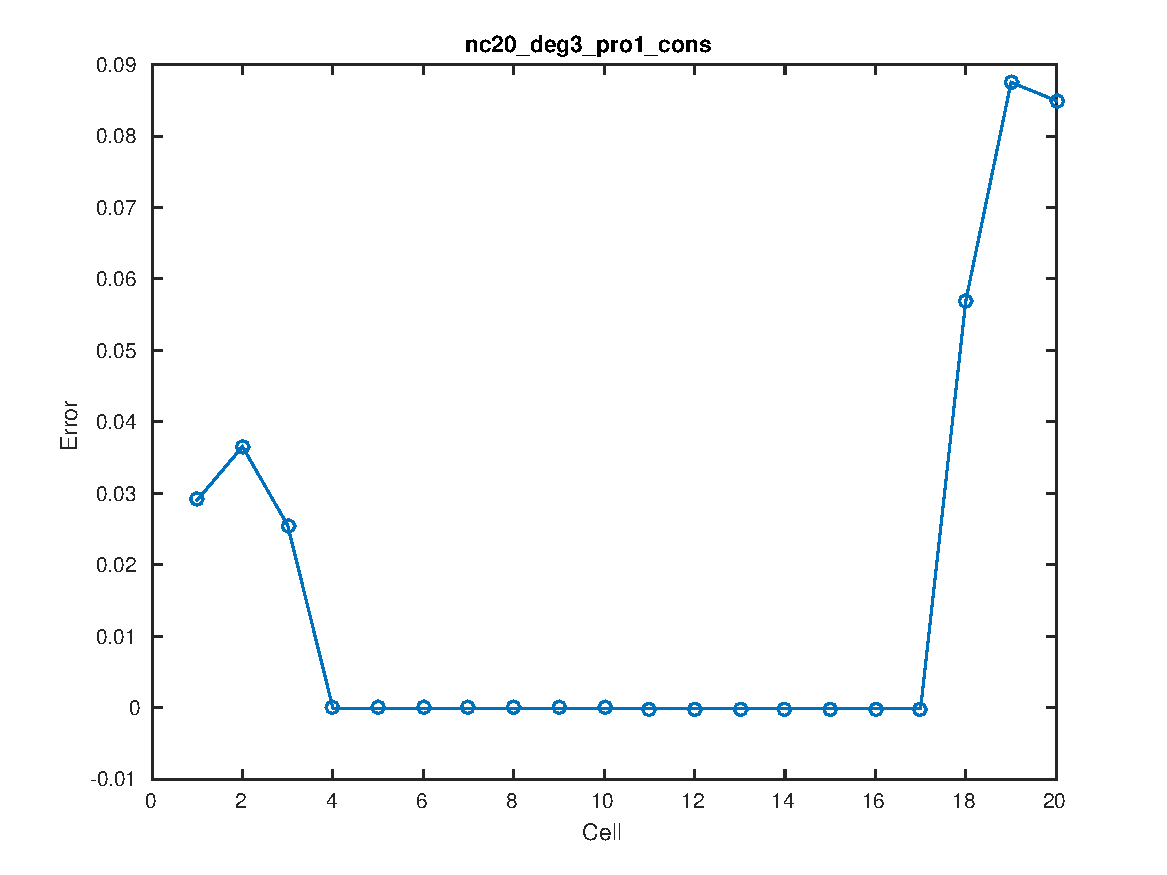
\includegraphics[width=\linewidth]{../../tests_01_01/test_01_01_test1_pro1_cons/output/plots/nc20_deg3_wei111_pro1_cons.pdf}
\end{subfigure}\hspace*{\fill}
\begin{subfigure}[b]{0.48\textwidth}
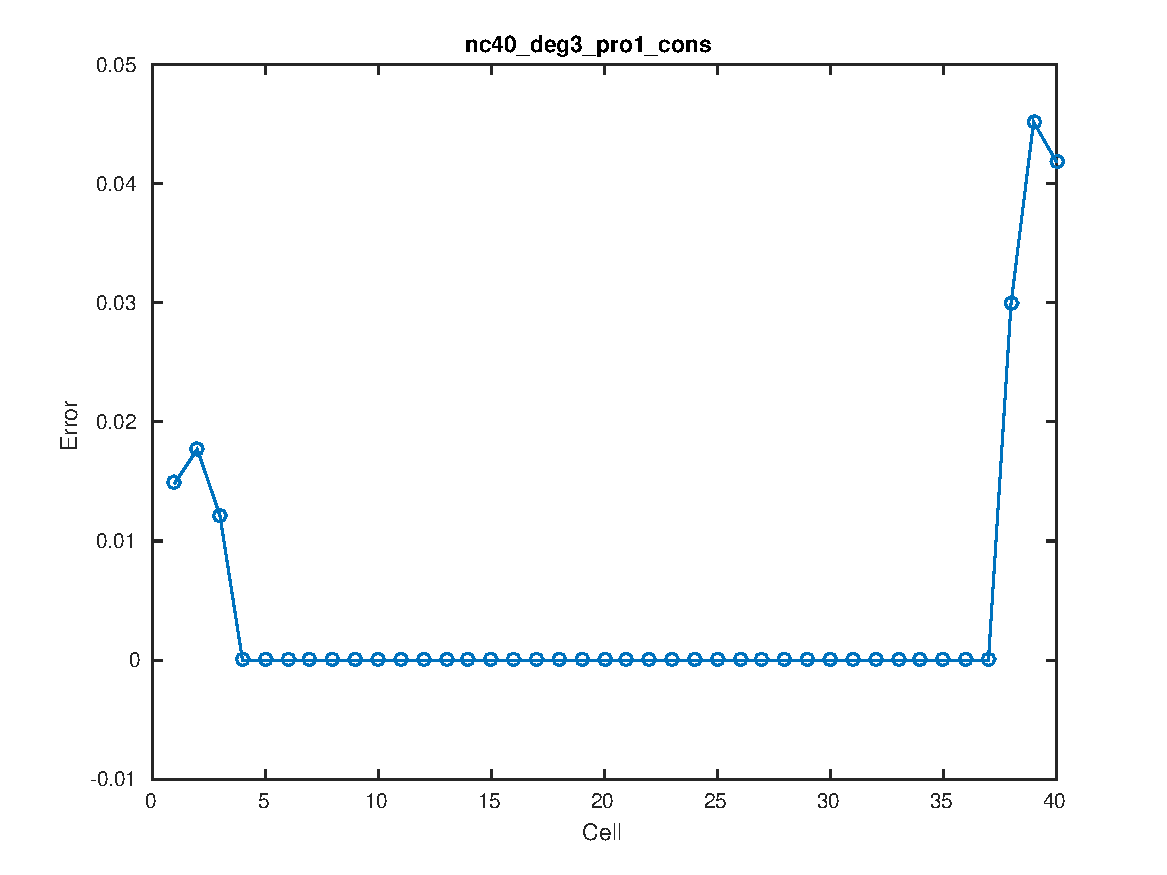
\includegraphics[width=\linewidth]{../../tests_01_01/test_01_01_test1_pro1_cons/output/plots/nc40_deg3_wei111_pro1_cons.pdf}
\end{subfigure}

\medskip
\begin{subfigure}[b]{0.48\textwidth}
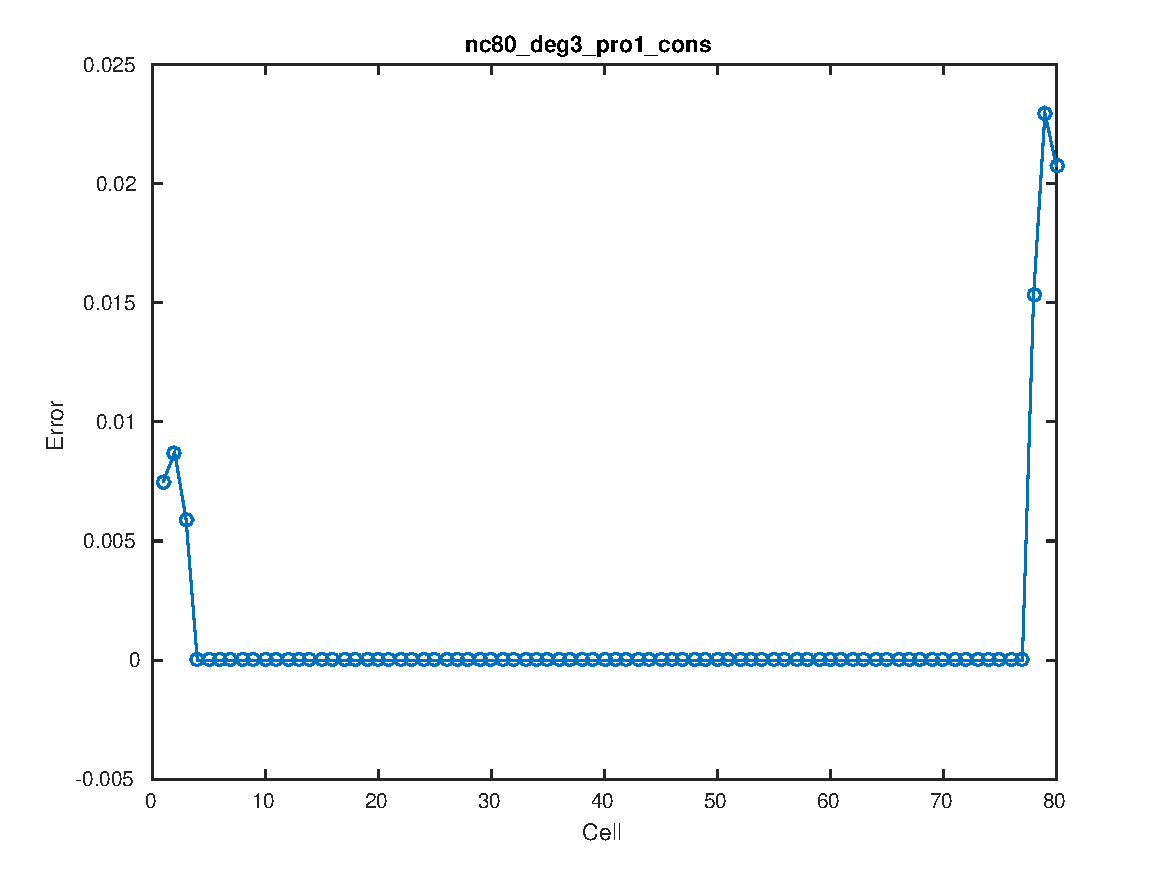
\includegraphics[width=\linewidth]{../../tests_01_01/test_01_01_test1_pro1_cons/output/plots/nc80_deg3_wei111_pro1_cons.pdf}
\end{subfigure}\hspace*{\fill}
\begin{subfigure}[b]{0.48\textwidth}
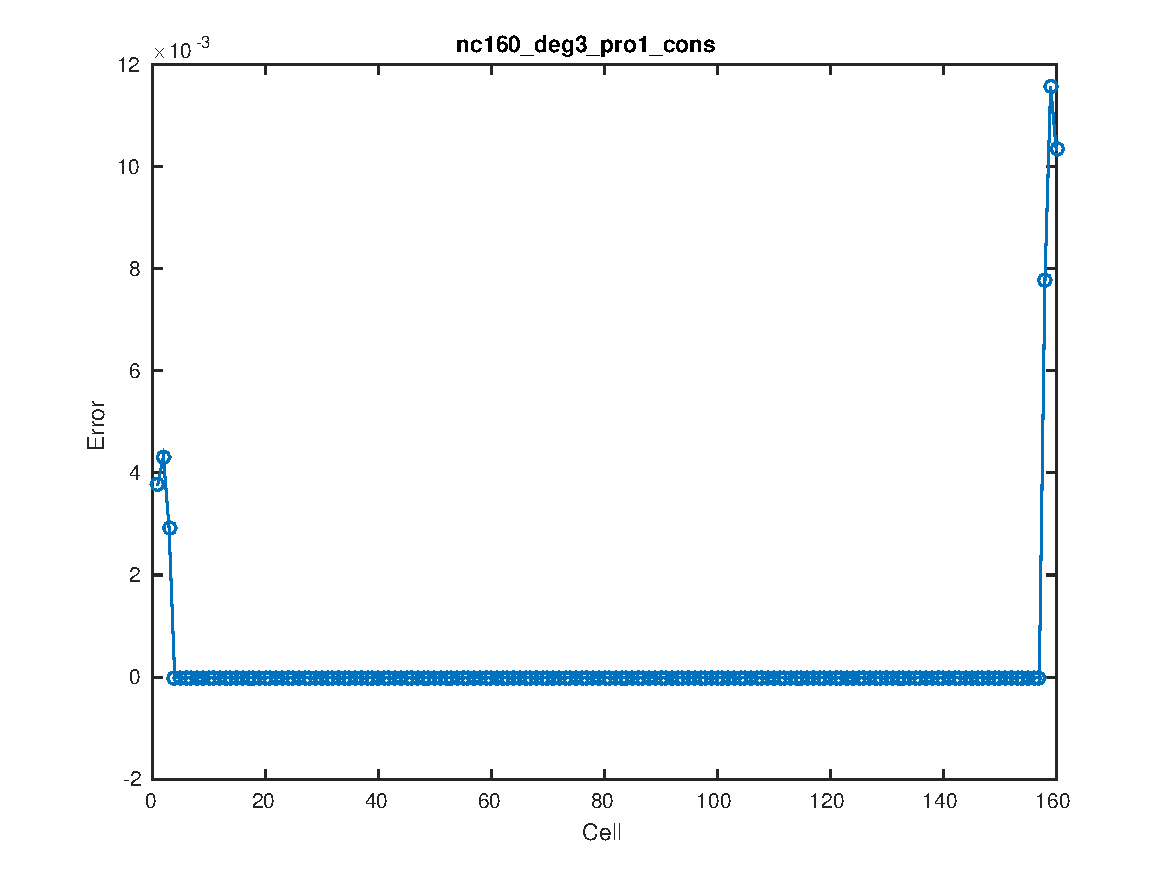
\includegraphics[width=\linewidth]{../../tests_01_01/test_01_01_test1_pro1_cons/output/plots/nc160_deg3_wei111_pro1_cons.pdf}
\end{subfigure}

\medskip
\begin{subfigure}[b]{0.48\textwidth}
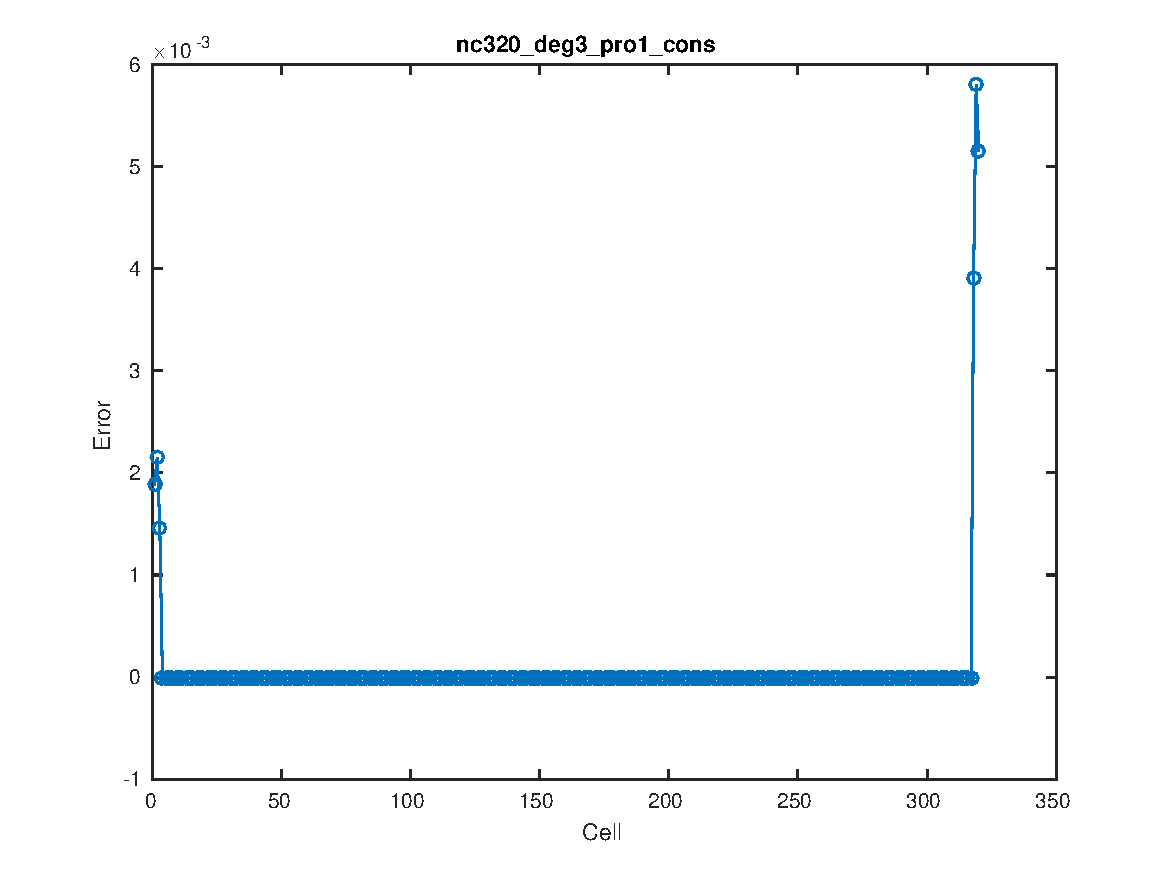
\includegraphics[width=\linewidth]{../../tests_01_01/test_01_01_test1_pro1_cons/output/plots/nc320_deg3_wei111_pro1_cons.pdf}
\end{subfigure}\hspace*{\fill}
\begin{subfigure}[b]{0.48\textwidth}
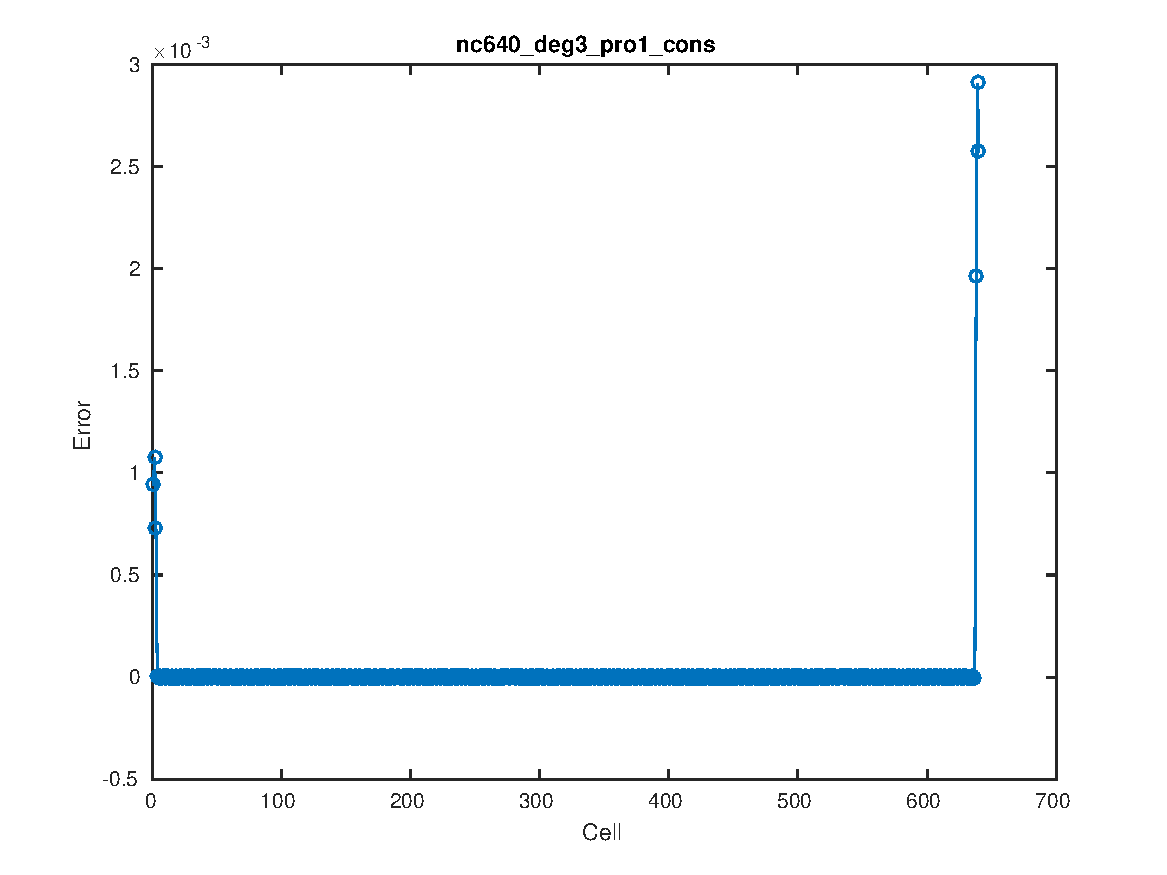
\includegraphics[width=\linewidth]{../../tests_01_01/test_01_01_test1_pro1_cons/output/plots/nc640_deg3_wei111_pro1_cons.pdf}
\end{subfigure}

\caption{$\omega=1|1,1$, d=3 (consistency)}
\end{figure}
%%% 3
\begin{figure}[H]
\begin{subfigure}[b]{0.48\textwidth}
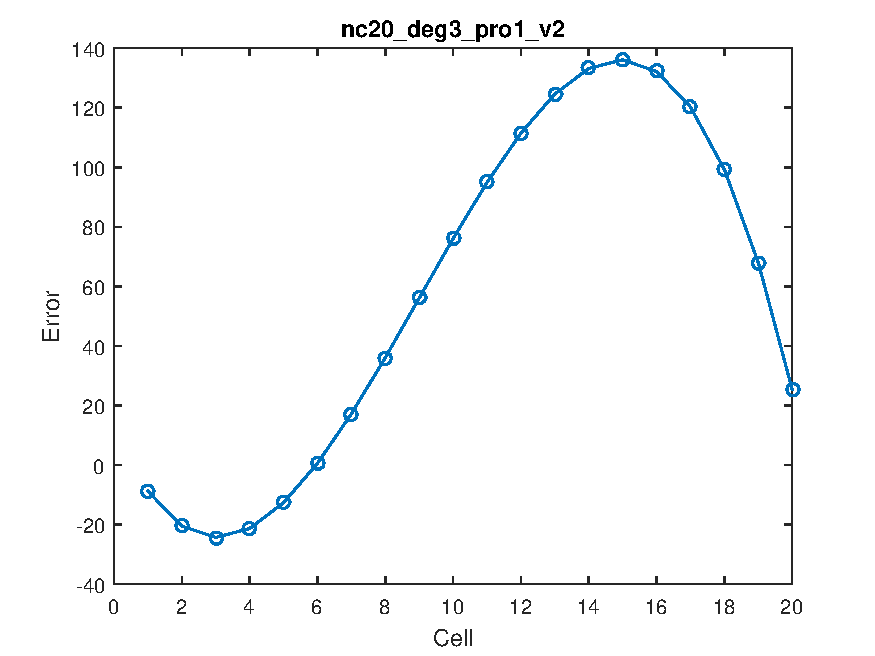
\includegraphics[width=\linewidth]{../../tests_01_01/test_01_01_test1_pro1/output/plots/nc20_deg3_wei111_pro1_v2.pdf}
\end{subfigure}\hspace*{\fill}
\begin{subfigure}[b]{0.48\textwidth}
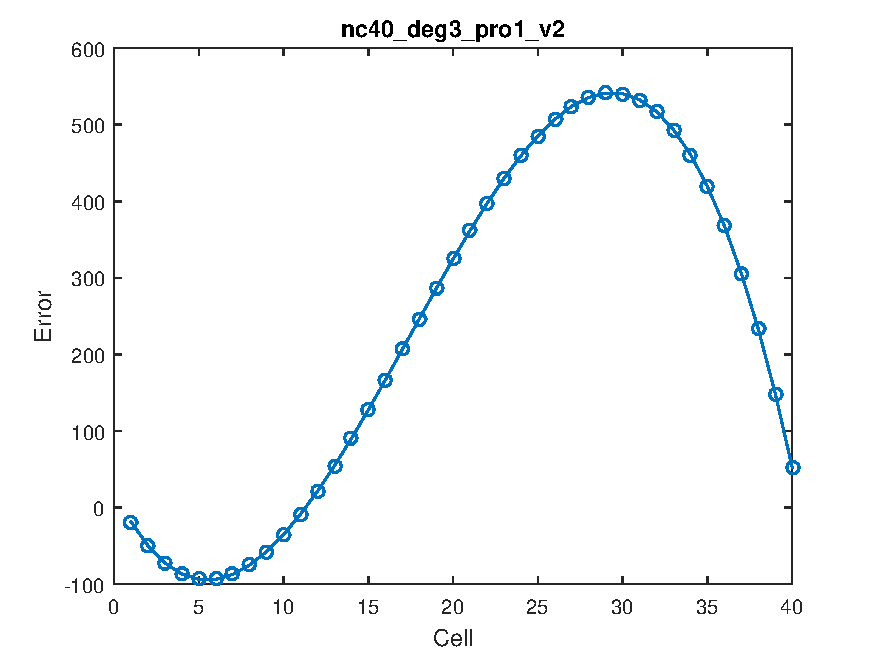
\includegraphics[width=\linewidth]{../../tests_01_01/test_01_01_test1_pro1/output/plots/nc40_deg3_wei111_pro1_v2.pdf}
\end{subfigure}

\medskip
\begin{subfigure}[b]{0.48\textwidth}
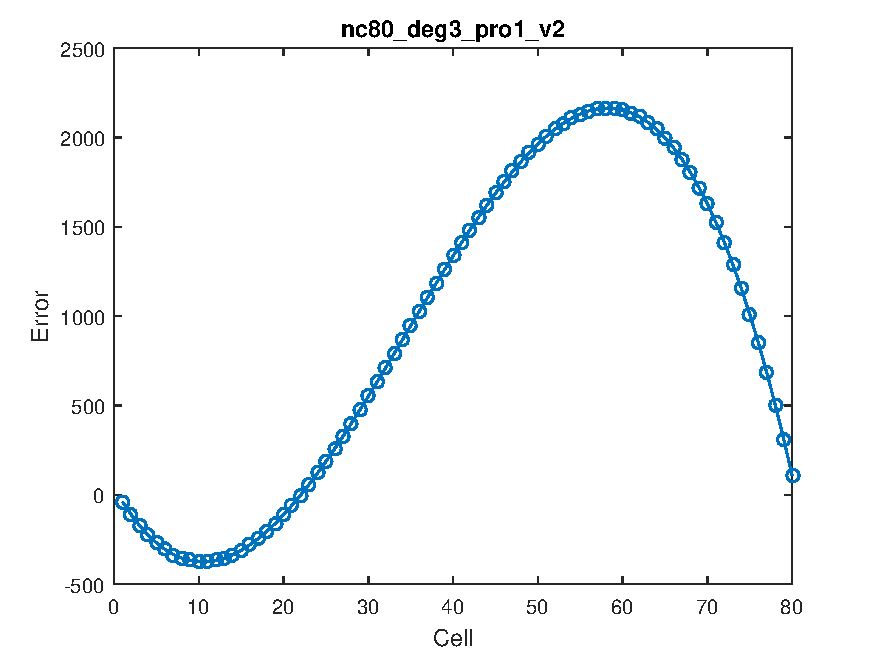
\includegraphics[width=\linewidth]{../../tests_01_01/test_01_01_test1_pro1/output/plots/nc80_deg3_wei111_pro1_v2.pdf}
\end{subfigure}\hspace*{\fill}
\begin{subfigure}[b]{0.48\textwidth}
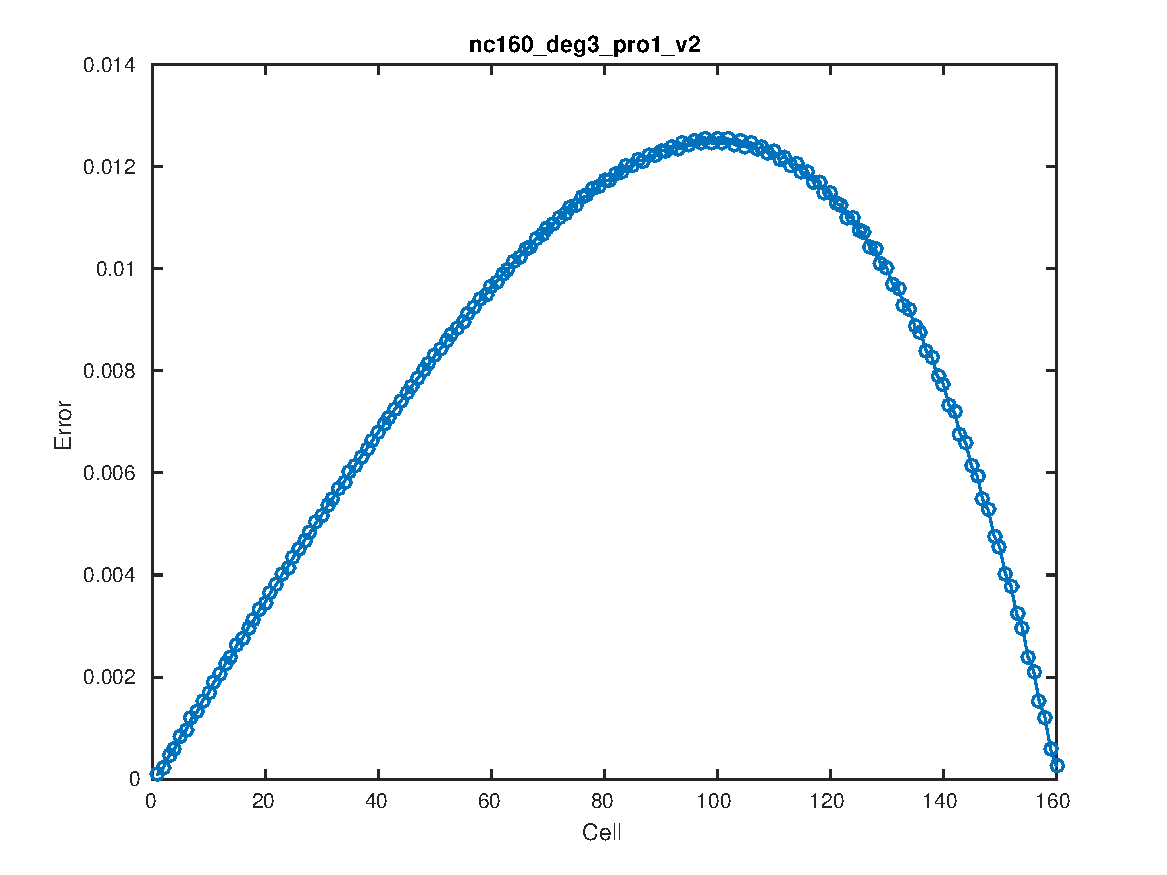
\includegraphics[width=\linewidth]{../../tests_01_01/test_01_01_test1_pro1/output/plots/nc160_deg3_wei111_pro1_v2.pdf}
\end{subfigure}

\medskip
\begin{subfigure}[b]{0.48\textwidth}
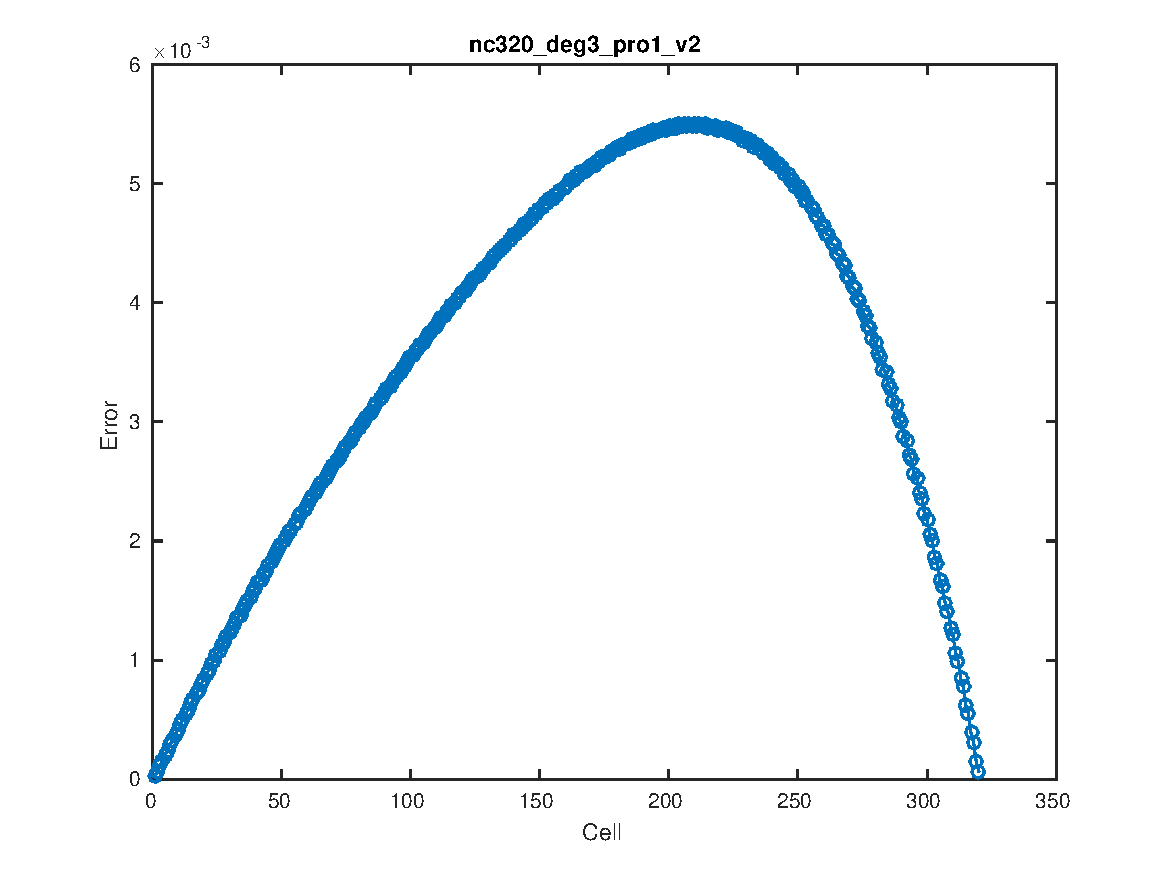
\includegraphics[width=\linewidth]{../../tests_01_01/test_01_01_test1_pro1/output/plots/nc320_deg3_wei111_pro1_v2.pdf}
\end{subfigure}\hspace*{\fill}
\begin{subfigure}[b]{0.48\textwidth}
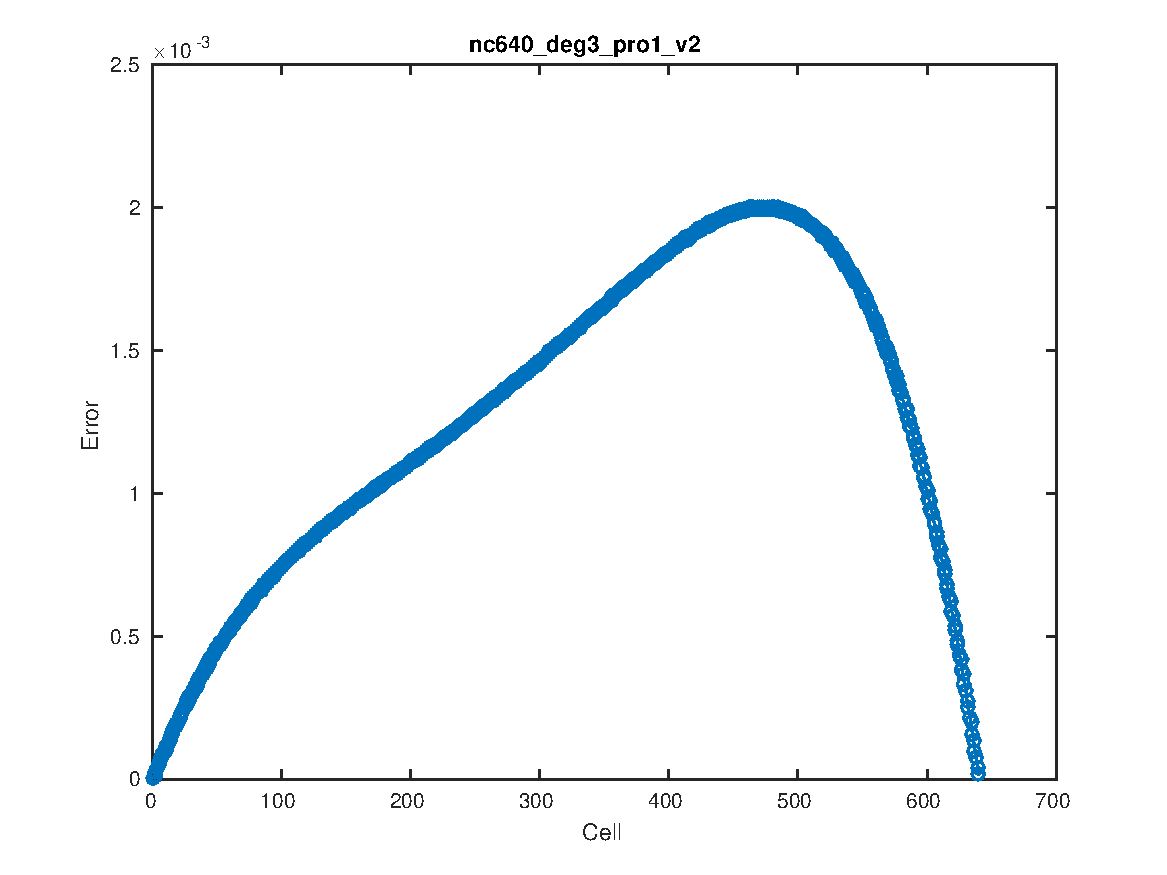
\includegraphics[width=\linewidth]{../../tests_01_01/test_01_01_test1_pro1/output/plots/nc640_deg3_wei111_pro1_v2.pdf}
\end{subfigure}

\caption{$\omega=1|1,1$, d=3  $\left(\frac{x-\overline{x}}{h^2}\right)$}
\end{figure}
\pagebreak
%%%%%%%%%%%%%%%%%%%%%%%%%%%%%%%%%%%%%%%%%%%%%%%%%%%%%%%%%%%%%%%%%%%%%%%%%%%%%%%%%%%%%%%%%%
In this tests we consider:
\begin{itemize}
\item $\psi(x)=\sin(\pi x)$
\item $\psi_\text l=0$
\item $\psi_\text{ll}=\pi$
\item $\psi_\text r=0$
\item $\psi_\text{rr}=-\pi$
\item $g(x)=-\pi^4\sin(\pi x)$
\end{itemize}
\begin{table}[H]
\setlength{\tabcolsep}{5pt}
\centering
\caption{Numerical results of PRO1 scheme.}
\resizebox{\linewidth}{!}{%
  \begin{tabular}{@{}l c c c c c c c c c c c c@{}}
\toprule
&  & \multicolumn{2}{c}{$\omega=1|1,1$} &  & \multicolumn{2}{c}{$\omega=1|3,1$} &  & \multicolumn{2}{c}{$\omega=1|3,3$} &  & \multicolumn{2}{c}{$\omega=1|3,10$} \\
\cline{3-4} \cline{6-7} \cline{9-10} \cline{12-13}
 & $I$ & E$_{\infty,0}$ & O$_{\infty,0}$ &  & E$_{\infty,0}$ & O$_{\infty,0}$ &  & E$_{\infty,0}$ & O$_{\infty,0}$ &  & E$_{\infty,0}$ & O$_{\infty,0}$ \\
\midrule
\multirow{6}{*}{$\mathbb{P}_{3}$(4)}
 & 20 & 5.37E$-$03 & ---  &  & 4.42E$-$03 & --- &  & 4.42E$-$03 & --- &  & 4.42E$-$03 & ---\\
 & 40 & 7.55E$-$04 & 2.83  &  & 6.90E$-$04 & 2.68 &  & 6.90E$-$04 & 2.68 &  & 6.90E$-$04 & 2.68\\
 & 80 & 1.51E$-$04 & 2.32  &  & 1.47E$-$04 & 2.24 &  & 1.47E$-$04 & 2.24 &  & 1.47E$-$04 & 2.24\\
 & 160 & 3.53E$-$05 & 2.09  &  & 3.50E$-$05 & 2.07 &  & 3.50E$-$05 & 2.07 &  & 3.50E$-$05 & 2.07\\
 & 320 & 8.67E$-$06 & 2.02  &  & 8.65E$-$06 & 2.02 &  & 8.65E$-$06 & 2.02 &  & 8.65E$-$06 & 2.02\\
 & 640 & 2.14E$-$06 & 2.02  &  & 2.15E$-$06 & 2.01 &  & 2.16E$-$06 & 2.00 &  & 2.15E$-$06 & 2.01\\
\midrule
\multirow{6}{*}{$\mathbb{P}_{5}$(6)}
 & 20 & 2.68E$-$05 & ---  &  & 2.24E$-$05 & --- &  & 2.24E$-$05 & --- &  & 2.24E$-$05 & ---\\
 & 40 & 3.73E$-$07 & 6.17  &  & 4.59E$-$07 & 5.61 &  & 4.59E$-$07 & 5.61 &  & 4.59E$-$07 & 5.61\\
 & 80 & 5.88E$-$08 & 2.66  &  & 5.41E$-$08 & 3.08 &  & 5.42E$-$08 & 3.08 &  & 5.41E$-$08 & 3.08\\
 & 160 & 4.11E$-$09 & 3.84  &  & 3.93E$-$09 & 3.78 &  & 3.55E$-$09 & 3.93 &  & 3.75E$-$09 & 3.85\\
 & 320 & 4.63E$-$10 & 3.15  &  & 1.62E$-$09 & 1.28 &  & 2.64E$-$09 & 0.43 &  & 3.06E$-$10 & 3.61\\
 & 640 & 4.31E$-$08 & $\uparrow$  &  & 3.45E$-$09 & $\uparrow$ &  & 8.41E$-$09 & $\uparrow$ &  & 1.32E$-$08 & $\uparrow$\\
\bottomrule
\end{tabular}}
\label{PRO:bending:01_01_glob7_pro1}
\end{table}
 % falta escolher o nome do glob
\begin{table}[H]
\setlength{\tabcolsep}{5pt}
\centering
\caption{Numerical results of PRO1 scheme (consistency).}
\resizebox{\linewidth}{!}{%
  \begin{tabular}{@{}l c c c c c c c c c c c c@{}}
\toprule
&  & \multicolumn{2}{c}{$\omega=1|1,1$} &  & \multicolumn{2}{c}{$\omega=1|3,1$} &  & \multicolumn{2}{c}{$\omega=1|3,3$} &  & \multicolumn{2}{c}{$\omega=1|3,10$} \\
\cline{3-4} \cline{6-7} \cline{9-10} \cline{12-13}
 & $I$ & E$_{\infty,0}$ & O$_{\infty,0}$ &  & E$_{\infty,0}$ & O$_{\infty,0}$ &  & E$_{\infty,0}$ & O$_{\infty,0}$ &  & E$_{\infty,0}$ & O$_{\infty,0}$ \\
\midrule
\multirow{6}{*}{$\mathbb{P}_{3}$(4)}
 & 20 & 6.97E$-$01 & ---  &  & 6.79E$-$01 & --- &  & 6.79E$-$01 & --- &  & 6.79E$-$01 & ---\\
 & 40 & 1.74E$-$01 & 2.00  &  & 1.70E$-$01 & 2.00 &  & 1.70E$-$01 & 2.00 &  & 1.70E$-$01 & 2.00\\
 & 80 & 4.34E$-$02 & 2.00  &  & 4.25E$-$02 & 2.00 &  & 4.25E$-$02 & 2.00 &  & 4.25E$-$02 & 2.00\\
 & 160 & 1.08E$-$02 & 2.00  &  & 1.06E$-$02 & 2.00 &  & 1.06E$-$02 & 2.00 &  & 1.06E$-$02 & 2.00\\
 & 320 & 2.71E$-$03 & 2.00  &  & 2.65E$-$03 & 2.00 &  & 2.65E$-$03 & 2.00 &  & 2.65E$-$03 & 2.00\\
 & 640 & 6.78E$-$04 & 2.00  &  & 6.64E$-$04 & 2.00 &  & 6.64E$-$04 & 2.00 &  & 6.64E$-$04 & 2.00\\
\midrule
\multirow{6}{*}{$\mathbb{P}_{5}$(6)}
 & 20 & 5.18E$-$02 & ---  &  & 4.91E$-$02 & --- &  & 4.91E$-$02 & --- &  & 4.91E$-$02 & ---\\
 & 40 & 3.36E$-$03 & 3.95  &  & 3.18E$-$03 & 3.95 &  & 3.18E$-$03 & 3.95 &  & 3.18E$-$03 & 3.95\\
 & 80 & 2.12E$-$04 & 3.99  &  & 2.00E$-$04 & 3.99 &  & 2.00E$-$04 & 3.99 &  & 2.00E$-$04 & 3.99\\
 & 160 & 1.33E$-$05 & 4.00  &  & 1.26E$-$05 & 4.00 &  & 1.26E$-$05 & 4.00 &  & 1.25E$-$05 & 4.00\\
 & 320 & 8.50E$-$07 & 3.96  &  & 7.78E$-$07 & 4.01 &  & 8.18E$-$07 & 3.94 &  & 9.69E$-$07 & 3.69\\
 & 640 & 5.31E$-$07 & 0.68  &  & 1.04E$-$06 & $\uparrow$ &  & 5.68E$-$07 & 0.52 &  & 1.13E$-$06 & $\uparrow$\\
\bottomrule
\end{tabular}}
\label{PRO:bending:01_01_glob7_pro1_cons}
\end{table}


\begin{figure}[H]
\begin{subfigure}[b]{0.48\textwidth}
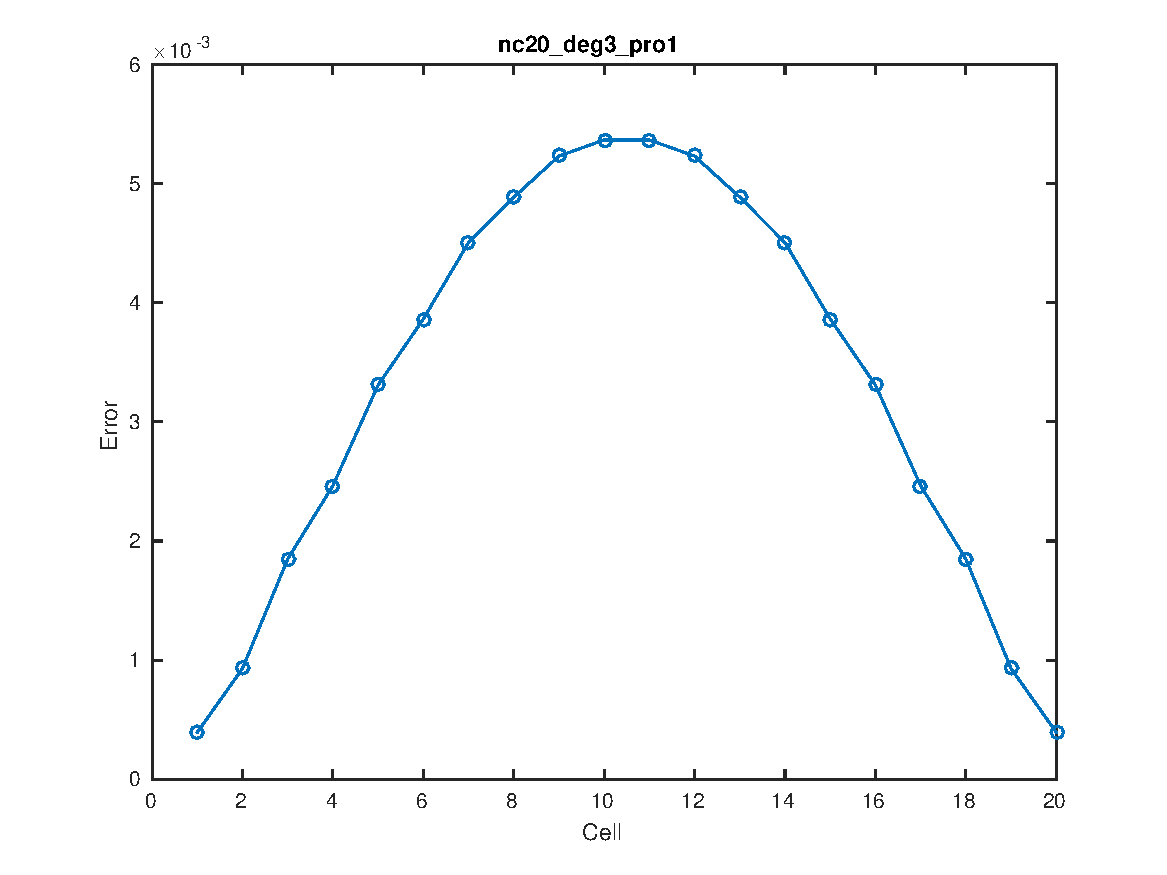
\includegraphics[width=\linewidth]{../../tests_01_01/test_01_01_test27_pro1/output/plots/nc20_deg3_wei111_pro1.pdf}
\end{subfigure}\hspace*{\fill}
\begin{subfigure}[b]{0.48\textwidth}
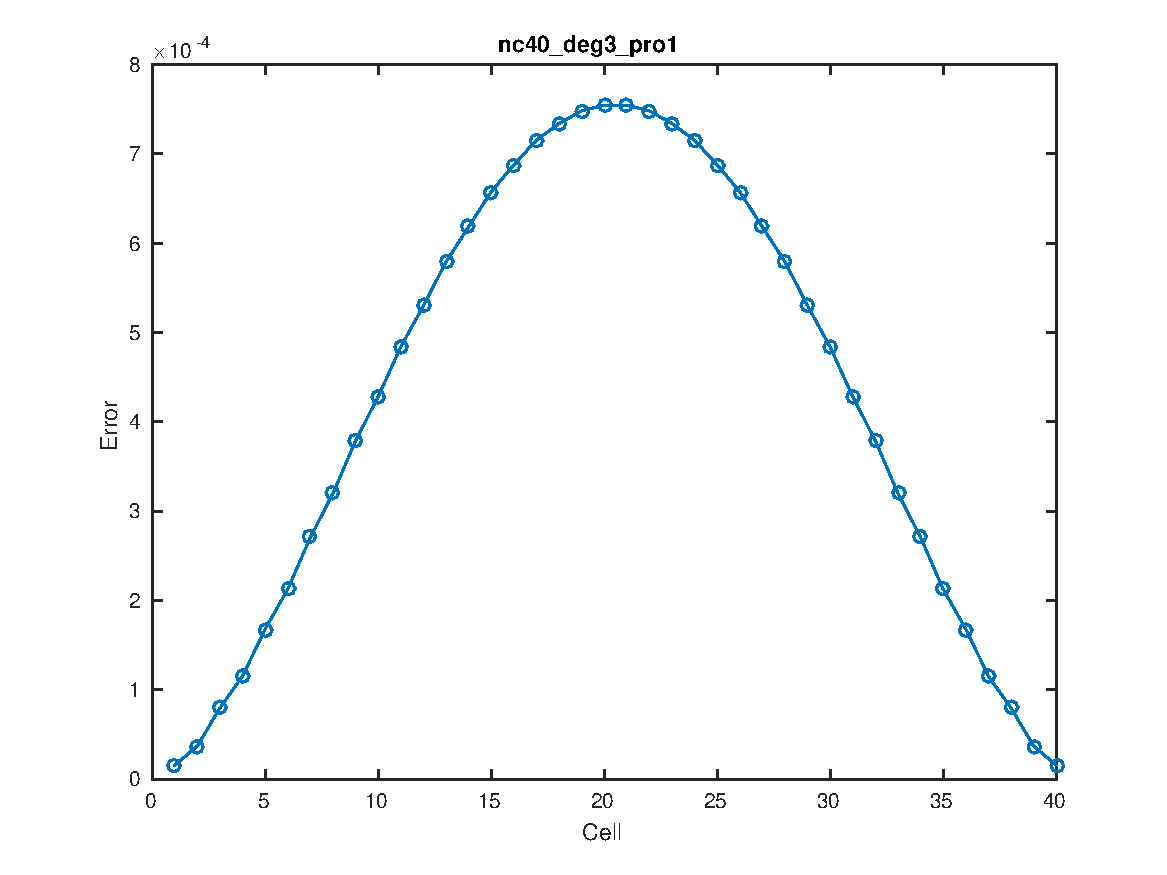
\includegraphics[width=\linewidth]{../../tests_01_01/test_01_01_test27_pro1/output/plots/nc40_deg3_wei111_pro1.pdf}
\end{subfigure}

\medskip
\begin{subfigure}[b]{0.48\textwidth}
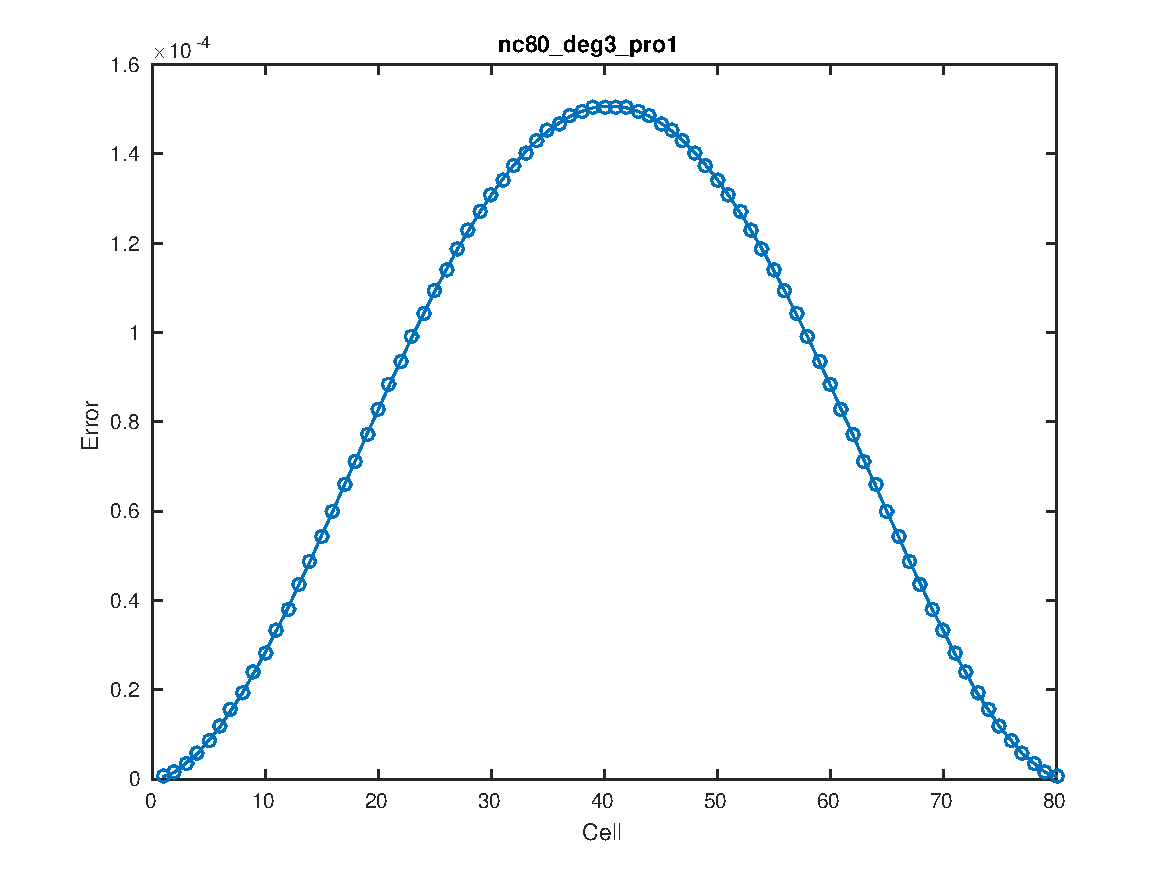
\includegraphics[width=\linewidth]{../../tests_01_01/test_01_01_test27_pro1/output/plots/nc80_deg3_wei111_pro1.pdf}
\end{subfigure}\hspace*{\fill}
\begin{subfigure}[b]{0.48\textwidth}
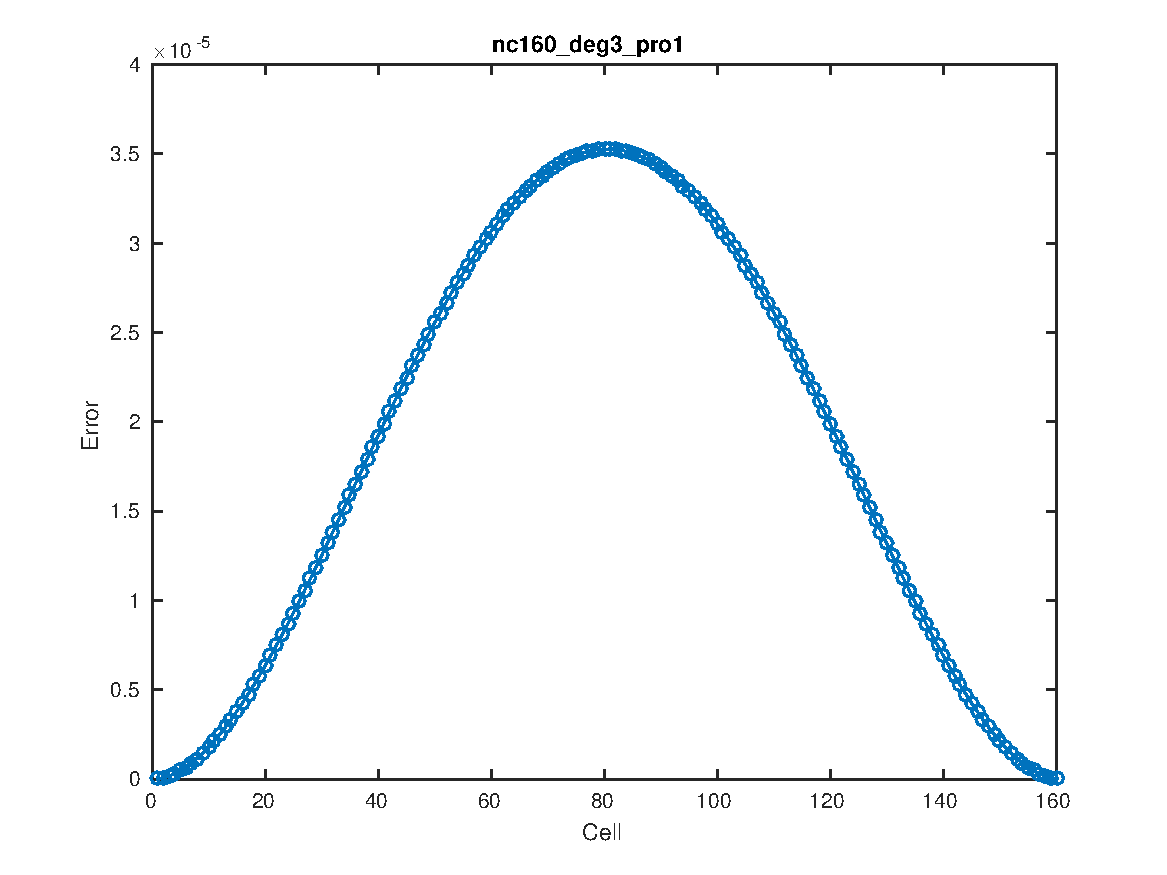
\includegraphics[width=\linewidth]{../../tests_01_01/test_01_01_test27_pro1/output/plots/nc160_deg3_wei111_pro1.pdf}
\end{subfigure}

\medskip
\begin{subfigure}[b]{0.48\textwidth}
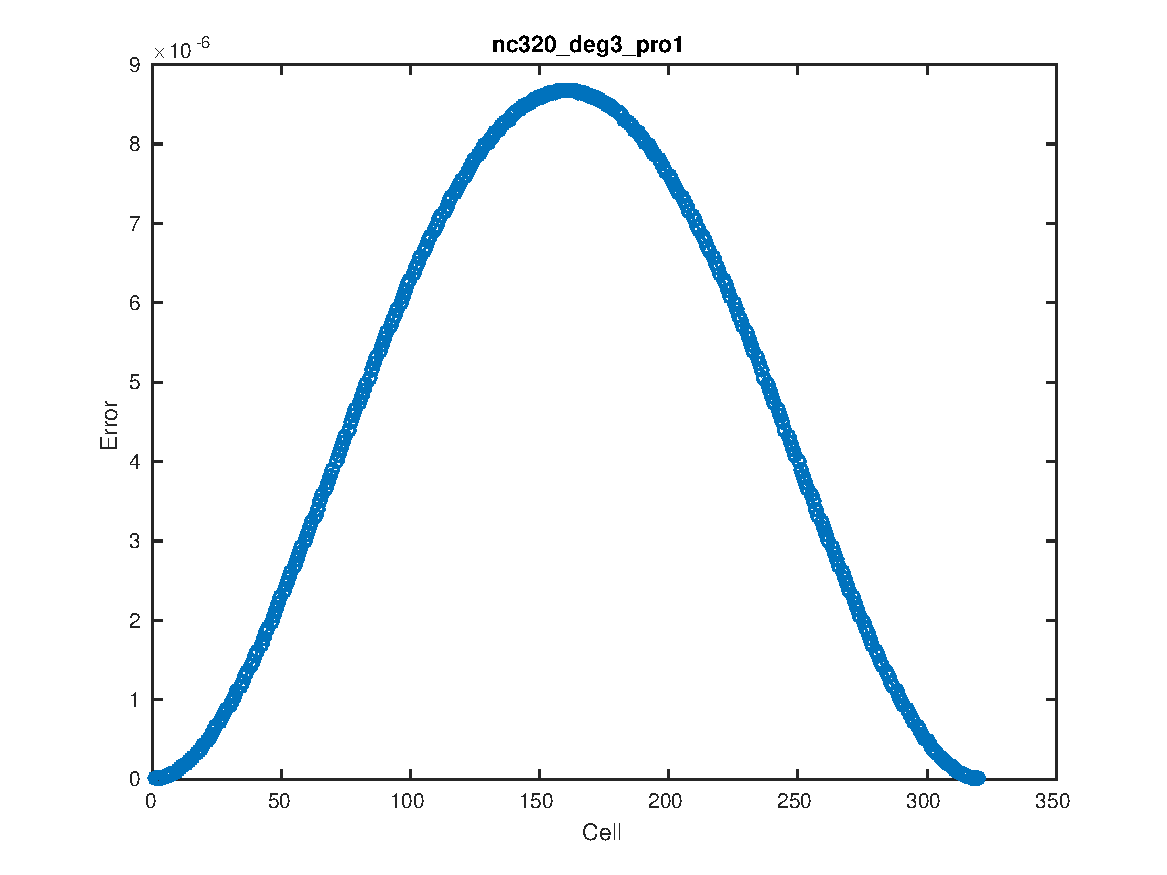
\includegraphics[width=\linewidth]{../../tests_01_01/test_01_01_test27_pro1/output/plots/nc320_deg3_wei111_pro1.pdf}
\end{subfigure}\hspace*{\fill}
\begin{subfigure}[b]{0.48\textwidth}
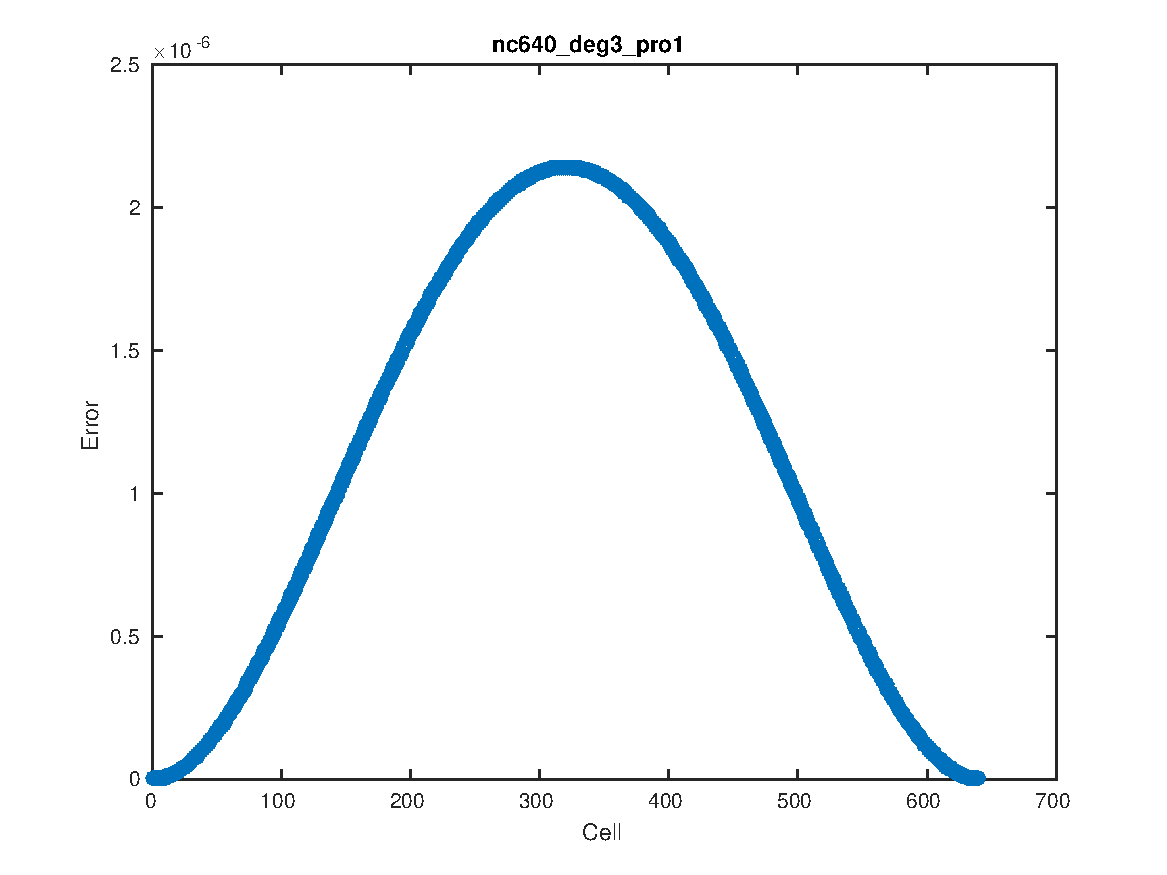
\includegraphics[width=\linewidth]{../../tests_01_01/test_01_01_test27_pro1/output/plots/nc640_deg3_wei111_pro1.pdf}
\end{subfigure}

\caption{$\omega=1|1,1$, d=3}
\end{figure}
%%% 2
\begin{figure}[H]
\begin{subfigure}[b]{0.48\textwidth}
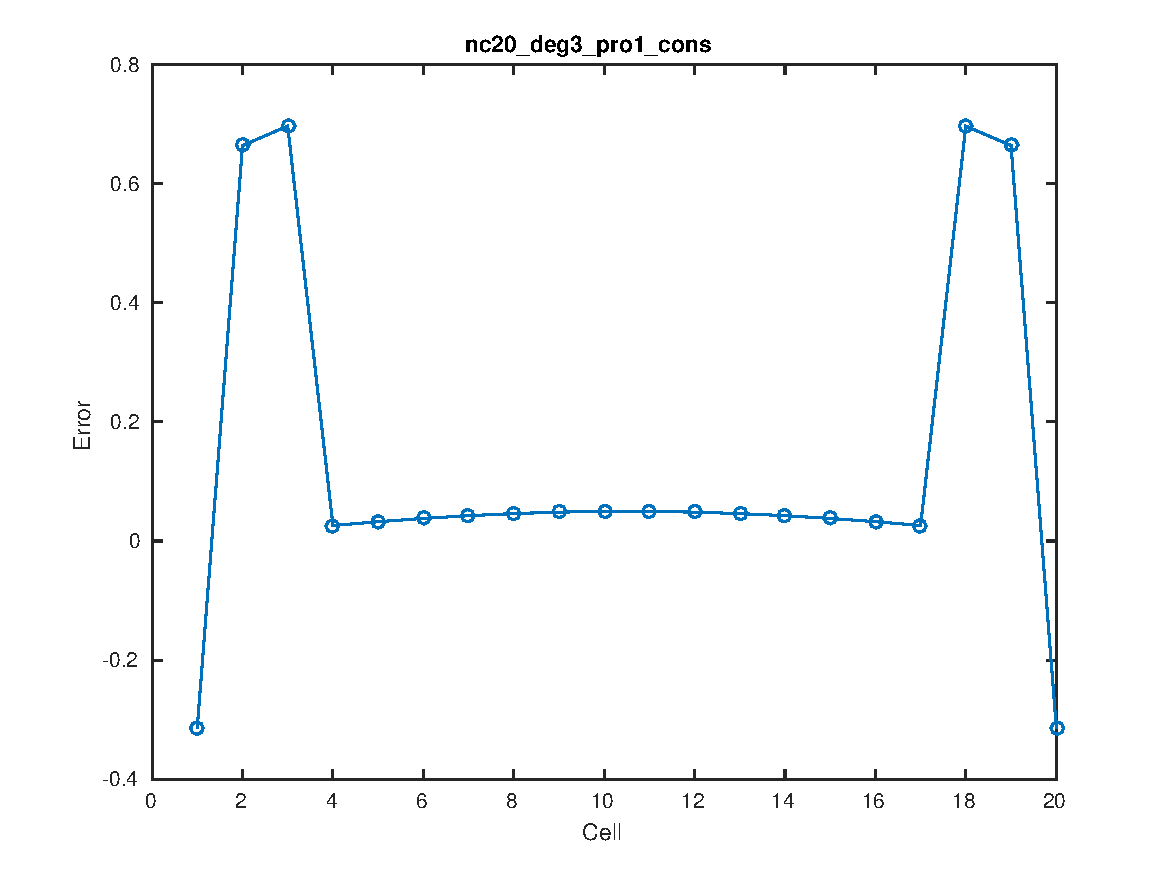
\includegraphics[width=\linewidth]{../../tests_01_01/test_01_01_test27_pro1_cons/output/plots/nc20_deg3_wei111_pro1_cons.pdf}
\end{subfigure}\hspace*{\fill}
\begin{subfigure}[b]{0.48\textwidth}
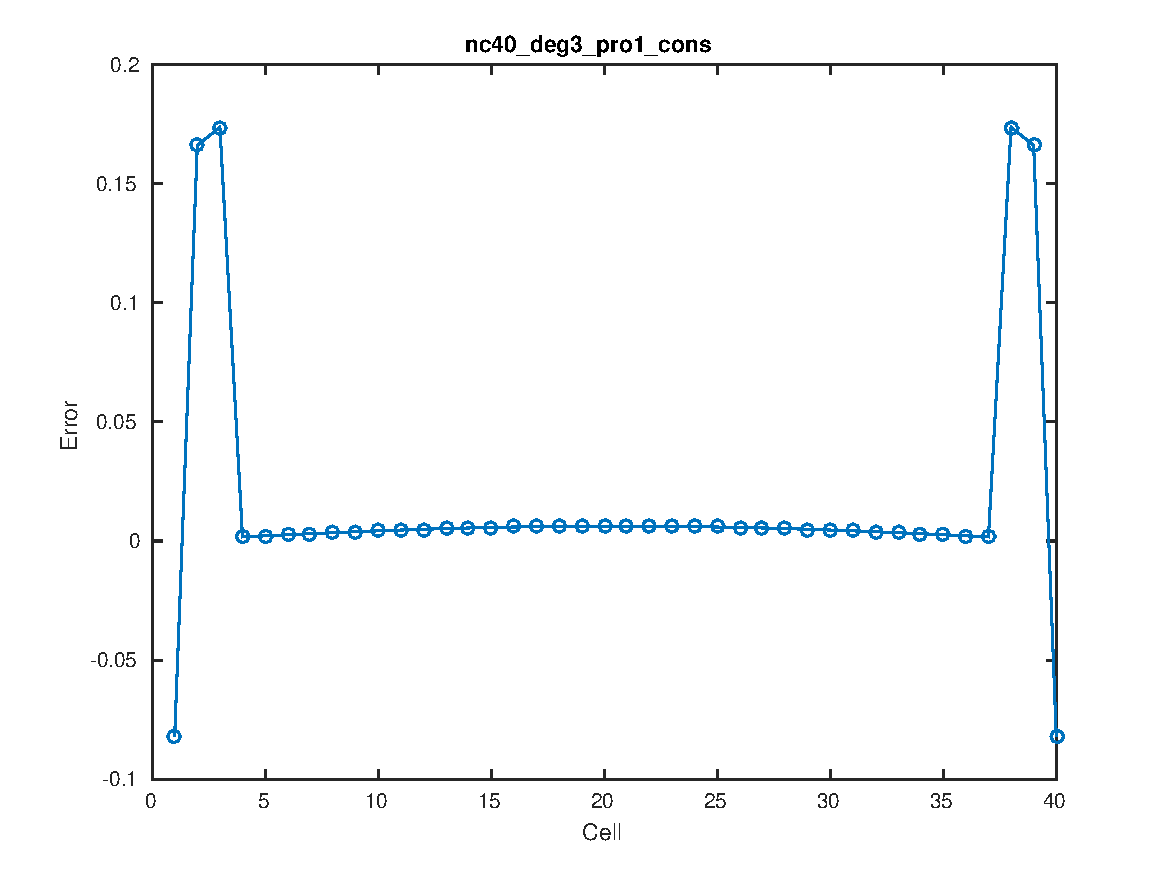
\includegraphics[width=\linewidth]{../../tests_01_01/test_01_01_test27_pro1_cons/output/plots/nc40_deg3_wei111_pro1_cons.pdf}
\end{subfigure}

\medskip
\begin{subfigure}[b]{0.48\textwidth}
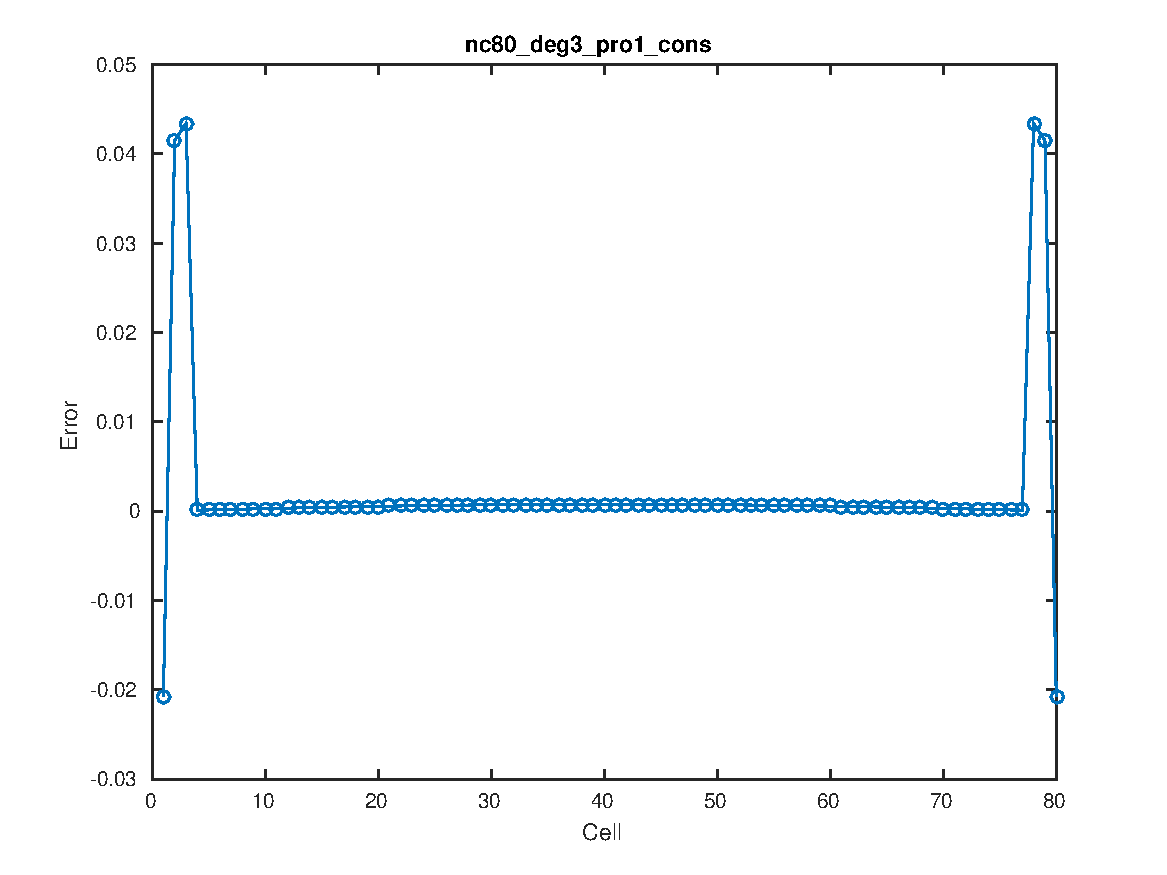
\includegraphics[width=\linewidth]{../../tests_01_01/test_01_01_test27_pro1_cons/output/plots/nc80_deg3_wei111_pro1_cons.pdf}
\end{subfigure}\hspace*{\fill}
\begin{subfigure}[b]{0.48\textwidth}
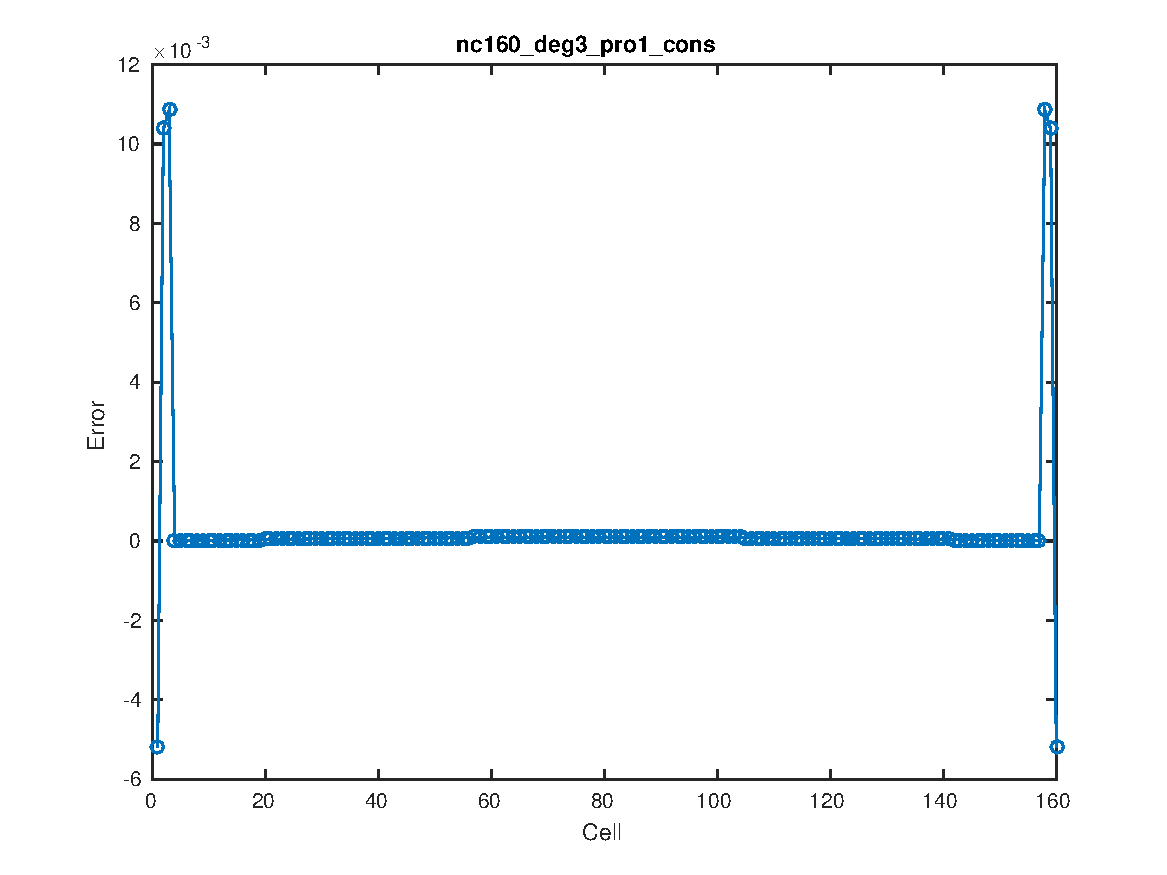
\includegraphics[width=\linewidth]{../../tests_01_01/test_01_01_test27_pro1_cons/output/plots/nc160_deg3_wei111_pro1_cons.pdf}
\end{subfigure}

\medskip
\begin{subfigure}[b]{0.48\textwidth}
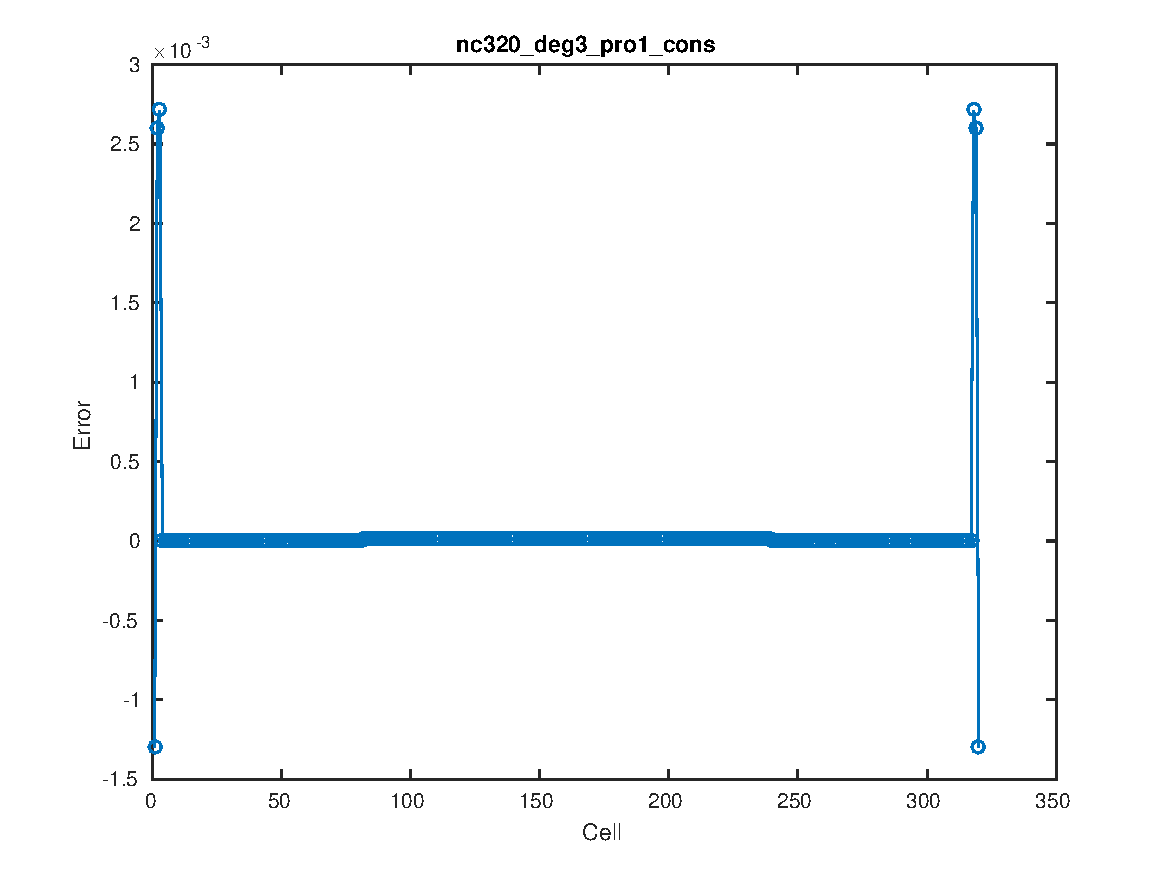
\includegraphics[width=\linewidth]{../../tests_01_01/test_01_01_test27_pro1_cons/output/plots/nc320_deg3_wei111_pro1_cons.pdf}
\end{subfigure}\hspace*{\fill}
\begin{subfigure}[b]{0.48\textwidth}
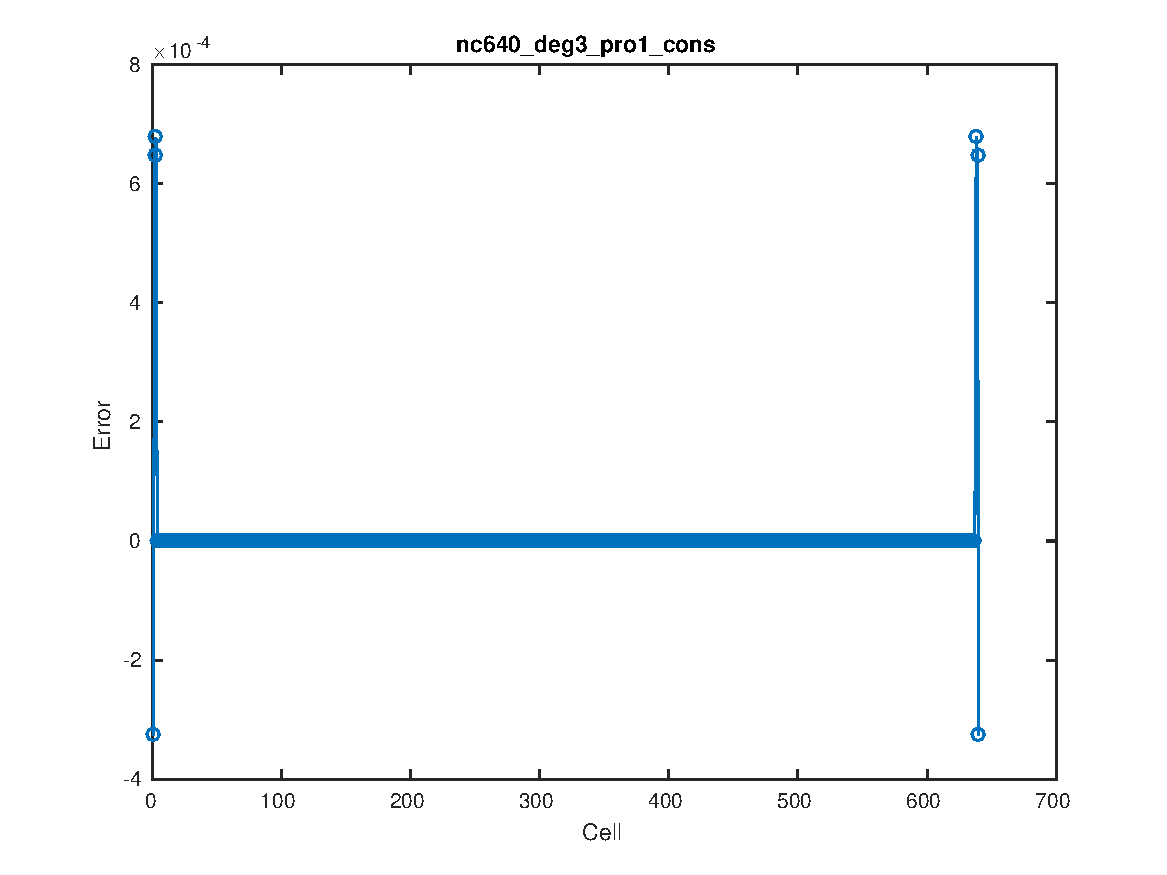
\includegraphics[width=\linewidth]{../../tests_01_01/test_01_01_test27_pro1_cons/output/plots/nc640_deg3_wei111_pro1_cons.pdf}
\end{subfigure}

\caption{$\omega=1|1,1$, d=3 (consistency)}
\end{figure}
%%% 3
\begin{figure}[H]
\begin{subfigure}[b]{0.48\textwidth}
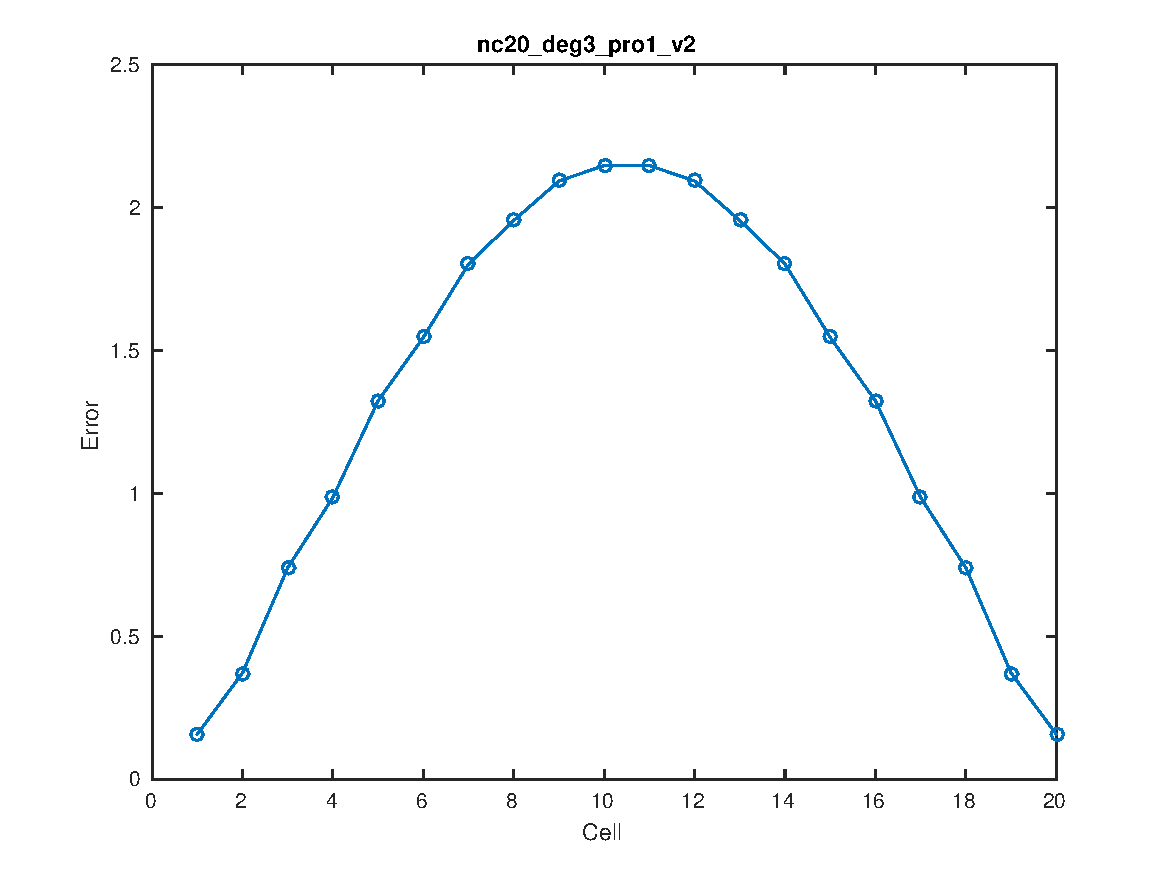
\includegraphics[width=\linewidth]{../../tests_01_01/test_01_01_test27_pro1/output/plots/nc20_deg3_wei111_pro1_v2.pdf}
\end{subfigure}\hspace*{\fill}
\begin{subfigure}[b]{0.48\textwidth}
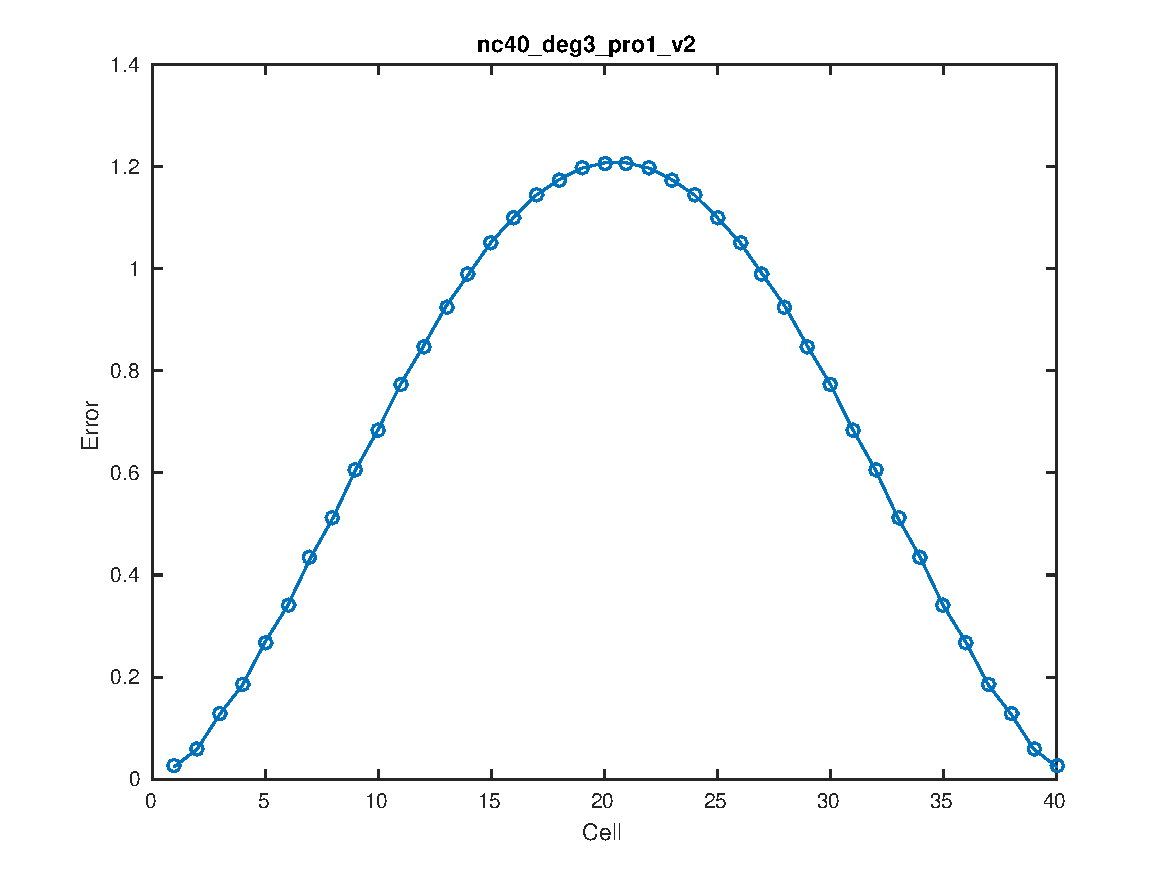
\includegraphics[width=\linewidth]{../../tests_01_01/test_01_01_test27_pro1/output/plots/nc40_deg3_wei111_pro1_v2.pdf}
\end{subfigure}

\medskip
\begin{subfigure}[b]{0.48\textwidth}
\includegraphics[width=\linewidth]{../../tests_01_01/test_01_01_test27_pro1/output/plots/nc80_deg3_wei111_pro1_v2.pdf}
\end{subfigure}\hspace*{\fill}
\begin{subfigure}[b]{0.48\textwidth}
\includegraphics[width=\linewidth]{../../tests_01_01/test_01_01_test27_pro1/output/plots/nc160_deg3_wei111_pro1_v2.pdf}
\end{subfigure}

\medskip
\begin{subfigure}[b]{0.48\textwidth}
\includegraphics[width=\linewidth]{../../tests_01_01/test_01_01_test27_pro1/output/plots/nc320_deg3_wei111_pro1_v2.pdf}
\end{subfigure}\hspace*{\fill}
\begin{subfigure}[b]{0.48\textwidth}
\includegraphics[width=\linewidth]{../../tests_01_01/test_01_01_test27_pro1/output/plots/nc640_deg3_wei111_pro1_v2.pdf}
\end{subfigure}

\caption{$\omega=1|1,1$, d=3 $\left(\frac{x-\overline{x}}{h^2}\right)$}
\end{figure}

\pagebreak
%%%%%%%%%%%%%%%%%%%%%%%%%%%%%%%%%%%%%%%%%%%%%%%%%%%%%%%%%%%%%%%%%%%%%%%%%%%%%%%%%%%%%%%%%%
In this tests we consider:
\begin{itemize}
\item $\psi(x)=-\exp(x)-(\text e-3)x^3-(5-2\text e)x^2+x+1$
\item $\psi_\text l=0$
\item $\psi_\text{ll}=0$
\item $\psi_\text r=0$
\item $\psi_\text{rr}=0$
\item $g(x)=\exp(x)$
\end{itemize}
\begin{table}[H]
\setlength{\tabcolsep}{5pt}
\centering
\caption{Numerical results of PRO1 scheme.}
\resizebox{\linewidth}{!}{%
  \begin{tabular}{@{}l c c c c c c c c c c c c@{}}
\toprule
&  & \multicolumn{2}{c}{$\omega=1|1,1$} &  & \multicolumn{2}{c}{$\omega=1|3,1$} &  & \multicolumn{2}{c}{$\omega=1|3,3$} &  & \multicolumn{2}{c}{$\omega=1|3,10$} \\
\cline{3-4} \cline{6-7} \cline{9-10} \cline{12-13}
 & $I$ & E$_{\infty,0}$ & O$_{\infty,0}$ &  & E$_{\infty,0}$ & O$_{\infty,0}$ &  & E$_{\infty,0}$ & O$_{\infty,0}$ &  & E$_{\infty,0}$ & O$_{\infty,0}$ \\
\midrule
\multirow{6}{*}{$\mathbb{P}_{3}$(4)}
 & 20 & 2.60E$-$04 & ---  &  & 2.07E$-$04 & --- &  & 2.07E$-$04 & --- &  & 2.06E$-$04 & ---\\
 & 40 & 3.35E$-$05 & 2.95  &  & 2.65E$-$05 & 2.96 &  & 2.65E$-$05 & 2.96 &  & 2.65E$-$05 & 2.96\\
 & 80 & 4.14E$-$06 & 3.02  &  & 3.27E$-$06 & 3.02 &  & 3.27E$-$06 & 3.02 &  & 3.27E$-$06 & 3.02\\
 & 160 & 4.90E$-$07 & 3.08  &  & 3.82E$-$07 & 3.10 &  & 3.82E$-$07 & 3.10 &  & 3.82E$-$07 & 3.10\\
 & 320 & 5.40E$-$08 & 3.18  &  & 4.03E$-$08 & 3.25 &  & 4.01E$-$08 & 3.25 &  & 4.11E$-$08 & 3.22\\
 & 640 & 1.07E$-$08 & 2.34  &  & 7.36E$-$09 & 2.45 &  & 6.71E$-$09 & 2.58 &  & 1.09E$-$08 & 1.91\\
\midrule
\multirow{6}{*}{$\mathbb{P}_{5}$(6)}
 & 20 & 1.78E$-$07 & ---  &  & 1.48E$-$07 & --- &  & 1.48E$-$07 & --- &  & 1.48E$-$07 & ---\\
 & 40 & 5.36E$-$09 & 5.05  &  & 4.46E$-$09 & 5.06 &  & 4.45E$-$09 & 5.06 &  & 4.45E$-$09 & 5.06\\
 & 80 & 1.54E$-$10 & 5.12  &  & 1.57E$-$10 & 4.82 &  & 1.58E$-$10 & 4.82 &  & 1.40E$-$10 & 4.99\\
 & 160 & 3.50E$-$11 & 2.14  &  & 1.11E$-$10 & 0.51 &  & 1.69E$-$10 & $\uparrow$ &  & 4.62E$-$10 & $\uparrow$\\
 & 320 & 1.77E$-$09 & $\uparrow$  &  & 1.18E$-$09 & $\uparrow$ &  & 4.14E$-$09 & $\uparrow$ &  & 1.60E$-$10 & 1.53\\
 & 640 & 1.09E$-$08 & $\uparrow$  &  & 2.60E$-$08 & $\uparrow$ &  & 3.89E$-$08 & $\uparrow$ &  & 1.19E$-$08 & $\uparrow$\\
\bottomrule
\end{tabular}}
\label{PRO:bending:01_01_glob10_pro1}
\end{table}
 % falta escolher o nome do glob
\begin{table}[H]
\setlength{\tabcolsep}{5pt}
\centering
\caption{Numerical results of PRO1 scheme (consistency).}
\resizebox{\linewidth}{!}{%
  \begin{tabular}{@{}l c c c c c c c c c c c c@{}}
\toprule
&  & \multicolumn{2}{c}{$\omega=1|1,1$} &  & \multicolumn{2}{c}{$\omega=1|3,1$} &  & \multicolumn{2}{c}{$\omega=1|3,3$} &  & \multicolumn{2}{c}{$\omega=1|3,10$} \\
\cline{3-4} \cline{6-7} \cline{9-10} \cline{12-13}
 & $I$ & E$_{\infty,0}$ & O$_{\infty,0}$ &  & E$_{\infty,0}$ & O$_{\infty,0}$ &  & E$_{\infty,0}$ & O$_{\infty,0}$ &  & E$_{\infty,0}$ & O$_{\infty,0}$ \\
\midrule
\multirow{6}{*}{$\mathbb{P}_{3}$(4)}
 & 20 & 8.75E$-$02 & ---  &  & 9.24E$-$02 & --- &  & 9.24E$-$02 & --- &  & 9.24E$-$02 & ---\\
 & 40 & 4.52E$-$02 & 0.95  &  & 4.58E$-$02 & 1.01 &  & 4.58E$-$02 & 1.01 &  & 4.58E$-$02 & 1.01\\
 & 80 & 2.29E$-$02 & 0.98  &  & 2.33E$-$02 & 0.98 &  & 2.33E$-$02 & 0.98 &  & 2.33E$-$02 & 0.98\\
 & 160 & 1.16E$-$02 & 0.99  &  & 1.17E$-$02 & 0.99 &  & 1.17E$-$02 & 0.99 &  & 1.17E$-$02 & 0.99\\
 & 320 & 5.81E$-$03 & 0.99  &  & 5.89E$-$03 & 0.99 &  & 5.89E$-$03 & 0.99 &  & 5.89E$-$03 & 0.99\\
 & 640 & 2.91E$-$03 & 1.00  &  & 2.95E$-$03 & 1.00 &  & 2.95E$-$03 & 1.00 &  & 2.95E$-$03 & 1.00\\
\midrule
\multirow{6}{*}{$\mathbb{P}_{5}$(6)}
 & 20 & 4.48E$-$04 & ---  &  & 4.68E$-$04 & --- &  & 4.68E$-$04 & --- &  & 4.68E$-$04 & ---\\
 & 40 & 5.84E$-$05 & 2.94  &  & 6.11E$-$05 & 2.94 &  & 6.11E$-$05 & 2.94 &  & 6.11E$-$05 & 2.94\\
 & 80 & 7.45E$-$06 & 2.97  &  & 7.81E$-$06 & 2.97 &  & 7.81E$-$06 & 2.97 &  & 7.81E$-$06 & 2.97\\
 & 160 & 9.18E$-$07 & 3.02  &  & 9.64E$-$07 & 3.02 &  & 9.64E$-$07 & 3.02 &  & 9.64E$-$07 & 3.02\\
 & 320 & 1.25E$-$07 & 2.87  &  & 1.63E$-$07 & 2.57 &  & 1.63E$-$07 & 2.57 &  & 1.63E$-$07 & 2.57\\
 & 640 & 8.45E$-$07 & $\uparrow$  &  & 7.96E$-$07 & $\uparrow$ &  & 7.96E$-$07 & $\uparrow$ &  & 7.96E$-$07 & $\uparrow$\\
\bottomrule
\end{tabular}}
\label{PRO:bending:01_01_glob10_pro1_cons}
\end{table}
 
%%% 1
\begin{figure}[H]
\begin{subfigure}[b]{0.48\textwidth}
\includegraphics[width=\linewidth]{../../tests_01_01/test_01_01_test39_pro1/output/plots/nc20_deg3_wei111_pro1.pdf}
\end{subfigure}\hspace*{\fill}
\begin{subfigure}[b]{0.48\textwidth}
\includegraphics[width=\linewidth]{../../tests_01_01/test_01_01_test39_pro1/output/plots/nc40_deg3_wei111_pro1.pdf}
\end{subfigure}

\medskip
\begin{subfigure}[b]{0.48\textwidth}
\includegraphics[width=\linewidth]{../../tests_01_01/test_01_01_test39_pro1/output/plots/nc80_deg3_wei111_pro1.pdf}
\end{subfigure}\hspace*{\fill}
\begin{subfigure}[b]{0.48\textwidth}
\includegraphics[width=\linewidth]{../../tests_01_01/test_01_01_test39_pro1/output/plots/nc160_deg3_wei111_pro1.pdf}
\end{subfigure}

\medskip
\begin{subfigure}[b]{0.48\textwidth}
\includegraphics[width=\linewidth]{../../tests_01_01/test_01_01_test39_pro1/output/plots/nc320_deg3_wei111_pro1.pdf}
\end{subfigure}\hspace*{\fill}
\begin{subfigure}[b]{0.48\textwidth}
\includegraphics[width=\linewidth]{../../tests_01_01/test_01_01_test39_pro1/output/plots/nc640_deg3_wei111_pro1.pdf}
\end{subfigure}

\caption{$\omega=1|1,1$, d=3}
\end{figure}
%%% 2
\begin{figure}[H]
\begin{subfigure}[b]{0.48\textwidth}
\includegraphics[width=\linewidth]{../../tests_01_01/test_01_01_test39_pro1_cons/output/plots/nc20_deg3_wei111_pro1_cons.pdf}
\end{subfigure}\hspace*{\fill}
\begin{subfigure}[b]{0.48\textwidth}
\includegraphics[width=\linewidth]{../../tests_01_01/test_01_01_test39_pro1_cons/output/plots/nc40_deg3_wei111_pro1_cons.pdf}
\end{subfigure}

\medskip
\begin{subfigure}[b]{0.48\textwidth}
\includegraphics[width=\linewidth]{../../tests_01_01/test_01_01_test39_pro1_cons/output/plots/nc80_deg3_wei111_pro1_cons.pdf}
\end{subfigure}\hspace*{\fill}
\begin{subfigure}[b]{0.48\textwidth}
\includegraphics[width=\linewidth]{../../tests_01_01/test_01_01_test39_pro1_cons/output/plots/nc160_deg3_wei111_pro1_cons.pdf}
\end{subfigure}

\medskip
\begin{subfigure}[b]{0.48\textwidth}
\includegraphics[width=\linewidth]{../../tests_01_01/test_01_01_test39_pro1_cons/output/plots/nc320_deg3_wei111_pro1_cons.pdf}
\end{subfigure}\hspace*{\fill}
\begin{subfigure}[b]{0.48\textwidth}
\includegraphics[width=\linewidth]{../../tests_01_01/test_01_01_test39_pro1_cons/output/plots/nc640_deg3_wei111_pro1_cons.pdf}
\end{subfigure}

\caption{$\omega=1|1,1$, d=3 (consistency)}
\end{figure}
%%% 3
\begin{figure}[H]
\begin{subfigure}[b]{0.48\textwidth}
\includegraphics[width=\linewidth]{../../tests_01_01/test_01_01_test39_pro1/output/plots/nc20_deg3_wei111_pro1_v2.pdf}
\end{subfigure}\hspace*{\fill}
\begin{subfigure}[b]{0.48\textwidth}
\includegraphics[width=\linewidth]{../../tests_01_01/test_01_01_test39_pro1/output/plots/nc40_deg3_wei111_pro1_v2.pdf}
\end{subfigure}

\medskip
\begin{subfigure}[b]{0.48\textwidth}
\includegraphics[width=\linewidth]{../../tests_01_01/test_01_01_test39_pro1/output/plots/nc80_deg3_wei111_pro1_v2.pdf}
\end{subfigure}\hspace*{\fill}
\begin{subfigure}[b]{0.48\textwidth}
\includegraphics[width=\linewidth]{../../tests_01_01/test_01_01_test39_pro1/output/plots/nc160_deg3_wei111_pro1_v2.pdf}
\end{subfigure}

\medskip
\begin{subfigure}[b]{0.48\textwidth}
\includegraphics[width=\linewidth]{../../tests_01_01/test_01_01_test39_pro1/output/plots/nc320_deg3_wei111_pro1_v2.pdf}
\end{subfigure}\hspace*{\fill}
\begin{subfigure}[b]{0.48\textwidth}
\includegraphics[width=\linewidth]{../../tests_01_01/test_01_01_test39_pro1/output/plots/nc640_deg3_wei111_pro1_v2.pdf}
\end{subfigure}

\caption{$\omega=1|1,1$, d=3 $\left(\frac{x-\overline{x}}{h^2}\right)$}
\end{figure}
\pagebreak
%%%%%%%%%%%%%%%%%%%%%%%%%%%%%%%%%%%%%%%%%%%%%%%%%%%%%%%%%%%%%%%%%%%%%%%%%%%%%%%%%%%%%%%%%%
In this tests we consider:
\begin{itemize}
\item $\psi(x)=-\exp(x)-(\text e-3)x^3-(5-2\text e)x^2+1$
\item $\psi_\text l=0$
\item $\psi_\text{ll}=-1$
\item $\psi_\text r=-1$
\item $\psi_\text{rr}=-1$
\item $g(x)=\exp(x)$
\end{itemize}
\begin{table}[H]
\setlength{\tabcolsep}{5pt}
\centering
\caption{Numerical results of PRO1 scheme.}
\resizebox{\linewidth}{!}{%
  \begin{tabular}{@{}l c c c c c c c c c c c c@{}}
\toprule
&  & \multicolumn{2}{c}{$\omega=1|1,1$} &  & \multicolumn{2}{c}{$\omega=1|3,1$} &  & \multicolumn{2}{c}{$\omega=1|3,3$} &  & \multicolumn{2}{c}{$\omega=1|3,10$} \\
\cline{3-4} \cline{6-7} \cline{9-10} \cline{12-13}
 & $I$ & E$_{\infty,0}$ & O$_{\infty,0}$ &  & E$_{\infty,0}$ & O$_{\infty,0}$ &  & E$_{\infty,0}$ & O$_{\infty,0}$ &  & E$_{\infty,0}$ & O$_{\infty,0}$ \\
\midrule
\multirow{6}{*}{$\mathbb{P}_{3}$(4)}
 & 20 & 2.60E$-$04 & ---  &  & 2.07E$-$04 & --- &  & 2.07E$-$04 & --- &  & 2.06E$-$04 & ---\\
 & 40 & 3.35E$-$05 & 2.95  &  & 2.65E$-$05 & 2.96 &  & 2.65E$-$05 & 2.96 &  & 2.65E$-$05 & 2.96\\
 & 80 & 4.14E$-$06 & 3.02  &  & 3.27E$-$06 & 3.02 &  & 3.27E$-$06 & 3.02 &  & 3.27E$-$06 & 3.02\\
 & 160 & 4.90E$-$07 & 3.08  &  & 3.82E$-$07 & 3.10 &  & 3.82E$-$07 & 3.10 &  & 3.82E$-$07 & 3.10\\
 & 320 & 5.37E$-$08 & 3.19  &  & 4.08E$-$08 & 3.23 &  & 4.08E$-$08 & 3.23 &  & 4.08E$-$08 & 3.23\\
 & 640 & 5.07E$-$09 & 3.41  &  & 3.70E$-$09 & 3.46 &  & 3.70E$-$09 & 3.46 &  & 3.70E$-$09 & 3.46\\
\midrule
\multirow{6}{*}{$\mathbb{P}_{5}$(6)}
 & 20 & 1.78E$-$07 & ---  &  & 1.48E$-$07 & --- &  & 1.48E$-$07 & --- &  & 1.48E$-$07 & ---\\
 & 40 & 5.36E$-$09 & 5.05  &  & 4.46E$-$09 & 5.06 &  & 4.46E$-$09 & 5.06 &  & 4.46E$-$09 & 5.06\\
 & 80 & 1.55E$-$10 & 5.11  &  & 1.41E$-$10 & 4.98 &  & 1.41E$-$10 & 4.98 &  & 1.41E$-$10 & 4.98\\
 & 160 & 5.35E$-$12 & 4.86  &  & 5.51E$-$12 & 4.68 &  & 4.38E$-$12 & 5.01 &  & 4.88E$-$12 & 4.85\\
 & 320 & 1.16E$-$12 & 2.21  &  & 5.27E$-$12 & 0.06 &  & 6.54E$-$12 & $\uparrow$ &  & 4.27E$-$12 & 0.19\\
 & 640 & 1.67E$-$11 & $\uparrow$  &  & 8.64E$-$12 & $\uparrow$ &  & 1.03E$-$11 & $\uparrow$ &  & 1.87E$-$12 & 1.19\\
\bottomrule
\end{tabular}}
\label{PRO:bending:01_01_glob11_pro1}
\end{table}
 % falta escolher o nome do glob
\begin{table}[H]
\setlength{\tabcolsep}{5pt}
\centering
\caption{Numerical results of PRO1 scheme (consistency).}
\resizebox{\linewidth}{!}{%
  \begin{tabular}{@{}l c c c c c c c c c c c c@{}}
\toprule
&  & \multicolumn{2}{c}{$\omega=1|1,1$} &  & \multicolumn{2}{c}{$\omega=1|3,1$} &  & \multicolumn{2}{c}{$\omega=1|3,3$} &  & \multicolumn{2}{c}{$\omega=1|3,10$} \\
\cline{3-4} \cline{6-7} \cline{9-10} \cline{12-13}
 & $I$ & E$_{\infty,0}$ & O$_{\infty,0}$ &  & E$_{\infty,0}$ & O$_{\infty,0}$ &  & E$_{\infty,0}$ & O$_{\infty,0}$ &  & E$_{\infty,0}$ & O$_{\infty,0}$ \\
\midrule
\multirow{6}{*}{$\mathbb{P}_{3}$(4)}
 & 20 & 8.75E$-$02 & ---  &  & 9.24E$-$02 & --- &  & 9.24E$-$02 & --- &  & 9.24E$-$02 & ---\\
 & 40 & 4.52E$-$02 & 0.95  &  & 4.58E$-$02 & 1.01 &  & 4.58E$-$02 & 1.01 &  & 4.58E$-$02 & 1.01\\
 & 80 & 2.29E$-$02 & 0.98  &  & 2.33E$-$02 & 0.98 &  & 2.33E$-$02 & 0.98 &  & 2.33E$-$02 & 0.98\\
 & 160 & 1.16E$-$02 & 0.99  &  & 1.17E$-$02 & 0.99 &  & 1.17E$-$02 & 0.99 &  & 1.17E$-$02 & 0.99\\
 & 320 & 5.81E$-$03 & 0.99  &  & 5.89E$-$03 & 0.99 &  & 5.89E$-$03 & 0.99 &  & 5.89E$-$03 & 0.99\\
 & 640 & 2.91E$-$03 & 1.00  &  & 2.95E$-$03 & 1.00 &  & 2.95E$-$03 & 1.00 &  & 2.95E$-$03 & 1.00\\
\midrule
\multirow{6}{*}{$\mathbb{P}_{5}$(6)}
 & 20 & 4.48E$-$04 & ---  &  & 4.68E$-$04 & --- &  & 4.68E$-$04 & --- &  & 4.68E$-$04 & ---\\
 & 40 & 5.84E$-$05 & 2.94  &  & 6.11E$-$05 & 2.94 &  & 6.11E$-$05 & 2.94 &  & 6.11E$-$05 & 2.94\\
 & 80 & 7.45E$-$06 & 2.97  &  & 7.81E$-$06 & 2.97 &  & 7.81E$-$06 & 2.97 &  & 7.81E$-$06 & 2.97\\
 & 160 & 9.15E$-$07 & 3.03  &  & 9.59E$-$07 & 3.02 &  & 9.59E$-$07 & 3.03 &  & 9.63E$-$07 & 3.02\\
 & 320 & 9.31E$-$08 & 3.30  &  & 1.27E$-$07 & 2.92 &  & 1.30E$-$07 & 2.88 &  & 7.93E$-$08 & 3.60\\
 & 640 & 9.00E$-$07 & $\uparrow$  &  & 9.67E$-$07 & $\uparrow$ &  & 9.19E$-$07 & $\uparrow$ &  & 6.80E$-$07 & $\uparrow$\\
\bottomrule
\end{tabular}}
\label{PRO:bending:01_01_glob11_pro1_cons}
\end{table}
 
%%% 1
\begin{figure}[H]
\begin{subfigure}[b]{0.48\textwidth}
\includegraphics[width=\linewidth]{../../tests_01_01/test_01_01_test43_pro1/output/plots/nc20_deg3_wei111_pro1.pdf}
\end{subfigure}\hspace*{\fill}
\begin{subfigure}[b]{0.48\textwidth}
\includegraphics[width=\linewidth]{../../tests_01_01/test_01_01_test43_pro1/output/plots/nc40_deg3_wei111_pro1.pdf}
\end{subfigure}

\medskip
\begin{subfigure}[b]{0.48\textwidth}
\includegraphics[width=\linewidth]{../../tests_01_01/test_01_01_test43_pro1/output/plots/nc80_deg3_wei111_pro1.pdf}
\end{subfigure}\hspace*{\fill}
\begin{subfigure}[b]{0.48\textwidth}
\includegraphics[width=\linewidth]{../../tests_01_01/test_01_01_test43_pro1/output/plots/nc160_deg3_wei111_pro1.pdf}
\end{subfigure}

\medskip
\begin{subfigure}[b]{0.48\textwidth}
\includegraphics[width=\linewidth]{../../tests_01_01/test_01_01_test43_pro1/output/plots/nc320_deg3_wei111_pro1.pdf}
\end{subfigure}\hspace*{\fill}
\begin{subfigure}[b]{0.48\textwidth}
\includegraphics[width=\linewidth]{../../tests_01_01/test_01_01_test43_pro1/output/plots/nc640_deg3_wei111_pro1.pdf}
\end{subfigure}

\caption{$\omega=1|1,1$, d=3}
\end{figure}
%%% 2
\begin{figure}[H]
\begin{subfigure}[b]{0.48\textwidth}
\includegraphics[width=\linewidth]{../../tests_01_01/test_01_01_test43_pro1_cons/output/plots/nc20_deg3_wei111_pro1_cons.pdf}
\end{subfigure}\hspace*{\fill}
\begin{subfigure}[b]{0.48\textwidth}
\includegraphics[width=\linewidth]{../../tests_01_01/test_01_01_test43_pro1_cons/output/plots/nc40_deg3_wei111_pro1_cons.pdf}
\end{subfigure}

\medskip
\begin{subfigure}[b]{0.48\textwidth}
\includegraphics[width=\linewidth]{../../tests_01_01/test_01_01_test43_pro1_cons/output/plots/nc80_deg3_wei111_pro1_cons.pdf}
\end{subfigure}\hspace*{\fill}
\begin{subfigure}[b]{0.48\textwidth}
\includegraphics[width=\linewidth]{../../tests_01_01/test_01_01_test43_pro1_cons/output/plots/nc160_deg3_wei111_pro1_cons.pdf}
\end{subfigure}

\medskip
\begin{subfigure}[b]{0.48\textwidth}
\includegraphics[width=\linewidth]{../../tests_01_01/test_01_01_test43_pro1_cons/output/plots/nc320_deg3_wei111_pro1_cons.pdf}
\end{subfigure}\hspace*{\fill}
\begin{subfigure}[b]{0.48\textwidth}
\includegraphics[width=\linewidth]{../../tests_01_01/test_01_01_test43_pro1_cons/output/plots/nc640_deg3_wei111_pro1_cons.pdf}
\end{subfigure}

\caption{$\omega=1|1,1$, d=3 (consistency)}
\end{figure}
%%% 3
\begin{figure}[H]
\begin{subfigure}[b]{0.48\textwidth}
\includegraphics[width=\linewidth]{../../tests_01_01/test_01_01_test43_pro1/output/plots/nc20_deg3_wei111_pro1_v2.pdf}
\end{subfigure}\hspace*{\fill}
\begin{subfigure}[b]{0.48\textwidth}
\includegraphics[width=\linewidth]{../../tests_01_01/test_01_01_test43_pro1/output/plots/nc40_deg3_wei111_pro1_v2.pdf}
\end{subfigure}

\medskip
\begin{subfigure}[b]{0.48\textwidth}
\includegraphics[width=\linewidth]{../../tests_01_01/test_01_01_test43_pro1/output/plots/nc80_deg3_wei111_pro1_v2.pdf}
\end{subfigure}\hspace*{\fill}
\begin{subfigure}[b]{0.48\textwidth}
\includegraphics[width=\linewidth]{../../tests_01_01/test_01_01_test43_pro1/output/plots/nc160_deg3_wei111_pro1_v2.pdf}
\end{subfigure}

\medskip
\begin{subfigure}[b]{0.48\textwidth}
\includegraphics[width=\linewidth]{../../tests_01_01/test_01_01_test43_pro1/output/plots/nc320_deg3_wei111_pro1_v2.pdf}
\end{subfigure}\hspace*{\fill}
\begin{subfigure}[b]{0.48\textwidth}
\includegraphics[width=\linewidth]{../../tests_01_01/test_01_01_test43_pro1/output/plots/nc640_deg3_wei111_pro1_v2.pdf}
\end{subfigure}

\caption{$\omega=1|1,1$, d=3 $\left(\frac{x-\overline{x}}{h^2}\right)$}
\end{figure}
\end{document}
% end of file